\documentclass{article}
\usepackage[utf8]{inputenc}
\usepackage{graphicx}
\usepackage{hyperref}
\usepackage[T1]{fontenc}
\usepackage{tgbonum}

\title{Tic Tac Reflex Toe}

% \subtitle{A MADT 5274 CAPSTONE PROJECT II}

\author{
  \\\\ 
  Karayilanoglu , Dogukan \\ \texttt{C0755495}\\\\
  \and
  \\\\Pardillo , Rosette Lopez \\ \texttt{C0768425}\\\\\newline
}
\date{August 23 2020}
\begin{document}


\maketitle
~\\
% Project assets can be accessed from the following links:\\
~\newline
\begin{itemize}
    \item Github Link:\\ \url{https://github.com/otetLopez/TicTacReflexToe/}
    \item Video Demo:\\
    \url{https://github.com/otetLopez/TicTacReflexToe/Video}
    \item Google Site:\\
    \url{https://sites.google.com/view/tic-tac-reflex-toe/home}
    \item Latex Overleaf Link:\\
    \url{https://www.overleaf.com/read/jvysgmwscznm}
\end{itemize}
\newpage

\begin{abstract}
\centering
~\\
~\\
A MADT 5274 CAPSTONE PROJECT II BY TEAM \textbf{CRYPTO}
\end{abstract}
\newpage

\tableofcontents
\newpage

\listoffigures
\newpage





% ****** INTRODUCTION ******
\section{TEAM NAME: CRYPTO}
TEAM MEMBERS:
\begin{itemize}
    \item Dogukan Karayilanoglu C0755495
    \item Rosette Lopez Pardillo C0768425
\end{itemize}
~\newline
\section{Introduction}
    \textbf{\emph{Tic Tac Reflex Toe}} is a Tic Tac Toe mobile application game.
    \\\\
    \textit{Tic Tac Toe \emph{is also know as noughts and crosses, or Xs and Os is a strategical game for two players who take turns marking the spaces in a 3 by 3 grid.}}
    The player who succeeds in placing three of their marks in a horizontal, vertical, or diagonal row is the winner
    \\
    This document will discuss how Tic Tac Reflex Toe Development Plan.  
    
    \begin{itemize}
    	\item Implementation Design
    	\item Mobile Application Flow
    	\item Implementation Timeline
    	\item Acceptance Procedure
    	\item Tools and Technologies
    \end{itemize}
    ~\newline
    
    \subsection{Objective}
        As there are many Tic Tac Toe game applications available in the market, this project aims to be able to create a lite, simple, user-friendly, fun application Tic Tac Toe game.
        ~\\\\
        This project is also beneficial for the development members to fully understand real time applications which is an interesting and useful skill for a mobile application developer.
   \newpage

% ****** CONTEXT ****** 
\section{The Context of Study}
    This mobile application project aims to deliver a stable mobile application software that covers important features that are required for a Capstone-Level Project.
    \\\\
    This mobile application project will be implemented in IOS using Swift.
    \\\\
    Aside from its technical complexity, this mobile application project should allow developers to apply new knowledge namely, saving data into server, and Real-Time application.
    \\\\
    \textbf{\emph{Tic Tac Reflex Toe}} Mobile Application targets users which of different ages who like to play the classic Tic Tac Toe game.
    \\\\
    With \textbf{\emph{Tic Tac Reflex Toe}} Mobile Application handy and user friendly, the user can enjoy playing Tic Tac Toe, to anyone, anywhere, anytime, online or offline. 
    ~\\
% ****** DEFINING THE PROBLEM ****** 
\section{Defining and Analyzing the Problem}
    \textbf{\emph{Application Level.}} Tic Tac Toe game when played with highly intellectual players usually gets a draw.  
    \\\\
    \textbf{\emph{Development Knowledge Level.}} Development Members have no experience implementing a Real Time Application
    ~\\

% ****** THE PROPOSAL OF A SOLUTION ****** 
\section{The Proposal of a Solution}
    \textbf{\emph{Application Level.}}  \textbf{\emph{Tic Tac Reflex Toe}} refrains players to experience a draw, it is design to always declare a winner.\\\\
    \textbf{\emph{Development Knowledge Level.}}  Implement \textbf{\emph{Tic Tac Reflex Toe}}, making it real time to be enjoyed online by multiple players.
    ~\\
    \newpage

% ****** COMPETITIVE ANALYSIS ******  
\section{Competitive Analysis}
    \subsection{Strategy}
    Strategy of Tic Tac Reflex Toe game is differentiation. There are a lot of standardized tic tac to games on market.Our strategy is being different from  the rest to be able to compete or even doubled their download numbers.Differentiation will be provided by changing the nature of tic tac toe game, not the graphics.
    \subsection{Similar Applications}
    \begin{itemize}
        	\item Classic Tic Tac Toe Xs and Os
        	\item Noughts and Crosses
        	\item Tic Tac Toe
        	\item Draw Tic Tac Toe
        	\item Tic Tac Toe OXO
        	\item Tic Tac Toe x
        \end{itemize}
    
    \subsection{What makes Tic Tac Reflex Toe Unique}
    Standard Tic Tac Toe games can be drawn due to their nature and applications out there are all can be drawn. Tic Tac Reflex Toe will be unique by changing that behaviour, always there will be a winner at the end of the game and winner will be determined by measuring their reflexes which gives the name of the application.If game is draw, then a random dot will be appear on the screen for the user and who is touch that before than the opponent will be the winner.

\newpage
% ****** MARKETING PLAN ****** 
\section{Marketing Plan}
\subsection{Target Users}
    \textbf{\emph{Tic Tac Reflex Toe}} is for all ages.  Anyone with a smart mobile device who is up for games can play with this game.
\subsection{Network}
    \subsubsection{Social Media}
        In this Technological Era, Social Media is very influential.  The fact is, people tend to spend so much time online.  
        \newline
        \begin{itemize}
        	\item Facebook\\This page will advertise the application, give instructions and will give support to users who have queries
        	\item Instagram\\This account will advertise the application, give instructions and will give support to users who have queries
        	\item Twitter\\This account will advertise the application, give instructions and will give support to users who have queries
        	\item Youtube\\This channel will have tutorial videos, reviews and gameplay videos.
        \end{itemize}
    
    \subsubsection{Friends}
        Development Team's friends can share to their network about the \textbf{\emph{Tic Tac Reflex Toe}}. Friends can also share social media posts.  Social Media Influencer friends could also do shout outs to help advertise the app.
   \newpage
\subsection{Retaining User Engagement}
    Aside from offering a free cool app, to retain user engagement, \textbf{\emph{Tic Tac Reflex Toe}} development team aims to deliver a fast performing, zero-bug and easy-to-use application.\\\\
    Once available in the market, \textbf{\emph{Tic Tac Reflex Toe}} development team swears to be responsive in  App Store user comments.\\\\
    \textbf{\emph{Tic Tac Reflex Toe}} Support can also be reached 24 hours through email, Facebook, Instagram, Twitter, and Youtube.
    ~\newline

\subsection{Track User Engagement}
    \textbf{\emph{Tic Tac Reflex Toe}} development team will keep track on the application's market status.  Statistics will be monitored using tools.  User engagement will also be tracked by 
    checking user ratings and number of downloads.  These information can be retrieved in Apple’s App Store.  
    ~\newline
\subsection{Increasing User Engagement}
    \begin{itemize}
        \item \textbf{\emph{Tic Tac Reflex Toe}} will remain active in advertising in Social Media.
        \item \textbf{\emph{Tic Tac Reflex Toe}} will also have continuous updates for improvements and will remain responsive to user queries in both social media and application store.
    \end{itemize}
    
~\newpage
% ****** COST ****** 
\section{Cost}
    \subsection{Application}
        \textbf{\emph{Tic Tac Reflex Toe}} is free and for everyone to enjoy
    \subsection{Development} 
        This application will need two development resources to meet Aug 21, based on MADT 5247 timeline.  Initially, this will be implemented in IOS and deploying IOS application will need Apple Developer subscription that costs 299USD for organization.  Below is a rough estimation if this will be implemented by a small company. This estimation is upto delivery period only.  Support timeline is not included.
        \begin{figure}[h]
        \centering
        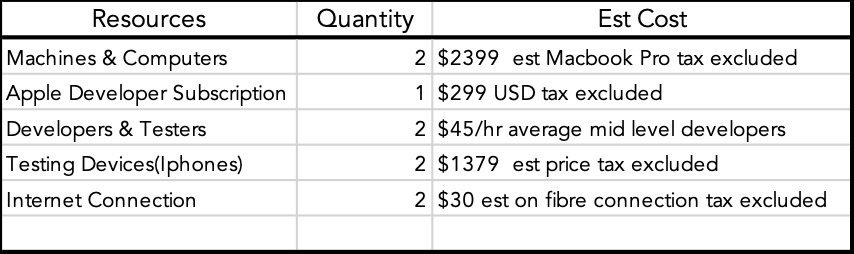
\includegraphics[width=5in]{images/Cost.jpg}
        \caption{Estimated Development Cost}
        \end{figure}
~\newline
% ****** MONETIZATION STRATEGY ****** 
\section{Monetization Strategy}
The very purpose of implementing \textbf{\emph{Tic Tac Reflex Toe}} is for the development team to learn developing real-time application.\\\\Thus this application is for FREE.\\\\And if \textbf{\emph{Tic Tac Reflex Toe}} will be a success, adding advertisements can be accepted.

~\newpage
% ****** APP FEATURES ******  
\section{App Features}
    \subsection{User Stories}
    \textbf{\emph{Tic Tac Reflex Toe}} is designed to support the following user stories:
    \begin{itemize}
        \item As a Mobile Development student, I want to learn to develop awesome real-time application
        \item As a user I want to play Tic Tac Toe online so I can play anywhere, anytime with online opponents
        \item As a user I want to play Tic Tac Toe digitally with a friend physically present
        \item As a user who plays Tic Tac Toe, I want to keep track of my score standing
        \item As a user, I want to log in into different devices so I can check my profile anytime
    \end{itemize}
    ~\\
    The following features are implemented to support the mentioned user stories above
    \begin{itemize}
    	\item \textbf{User Registration}\\
    	New user can register to enjoy playing the game.  User details needs to be inputted to be able to register successfully.
    	\item \textbf{User Profile}\\
    	Logged in user will be able to see his profile details in this page.
    	\item \textbf{Log In and Log Out}\\
    	User will be able to log in and log out using different devices.
    	\item \textbf{Dashboard}\\
    	This is the home page of the application.  This also shows online users list who are playing or who is available to play.
    	\item \textbf{Real-Time User Interaction}\\
    	Users will be able to enjoy playing the game with a real opponent as long as users are connected to the internet.
    	\item \textbf{Offline Mode}\\ 
    	User can play offline mode using only one device.
    	\item \textbf{User Game Standing}\\
    	The user can view user game standing.  This can be seen in User profile page.
    	\item \textbf{Notification}\\
    	Users that are being invited to play a game will be notified.
    \end{itemize}
    ~\newline

% ****** MOCKUP ****** 
\section{Use Cases}
    \subsection{Design}
        Below figure is a mock up on how the application is designed.\\ 
        \begin{figure}[h]
        \centering
        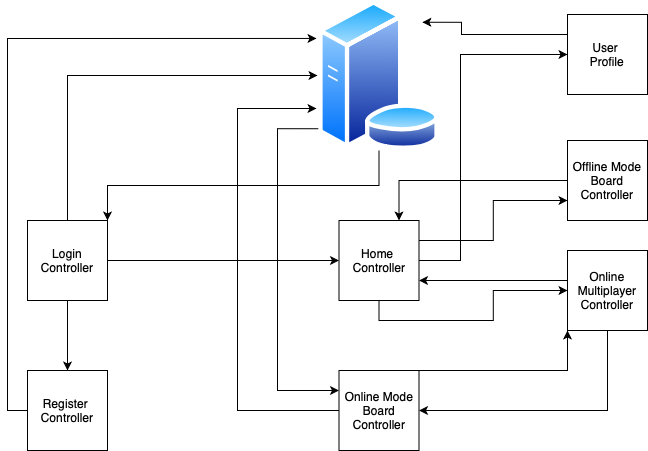
\includegraphics[width=5in]{images/tictacreflexdiagram.png}
        \caption{Application Mock Up}
        \end{figure}
        ~\newline
        ~\newpage
    
    \subsection{Layout}
        Below images shows the layout plan of how the application should look in an IPhone device.\\
        ~\newline
        \textbf{Log In Controller}
        \begin{figure}[h]
        \centering
        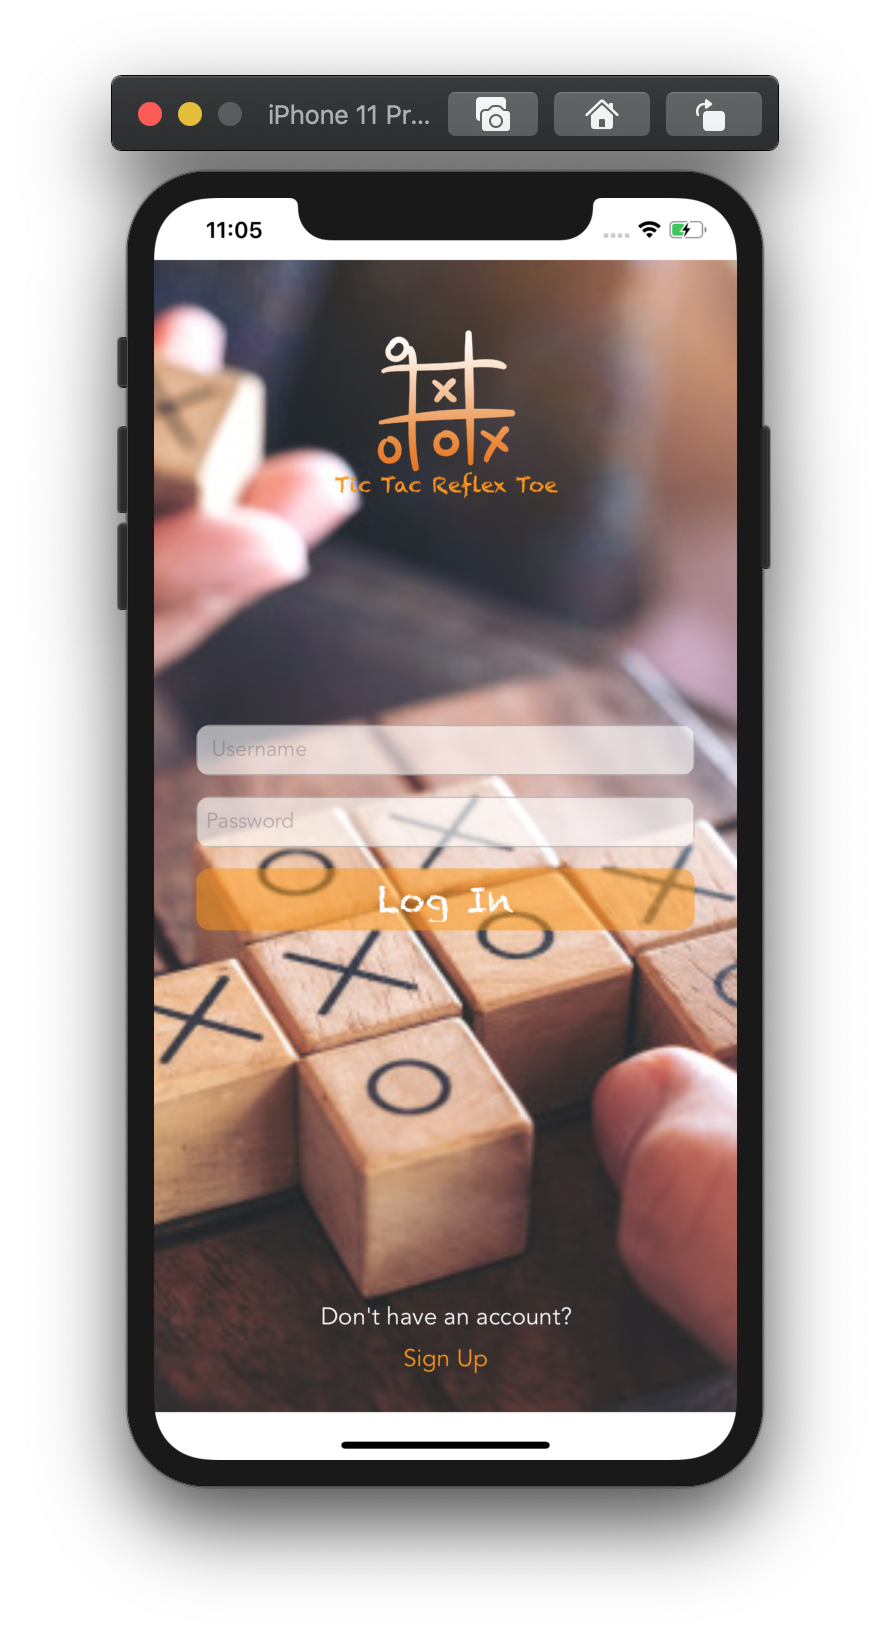
\includegraphics[width=3in]{images/login.png}
        \caption{Log In Page in Iphone}
        \end{figure}
        ~\newpage
        \textbf{Game Board Controller}
        \begin{figure}[h]
        \centering
        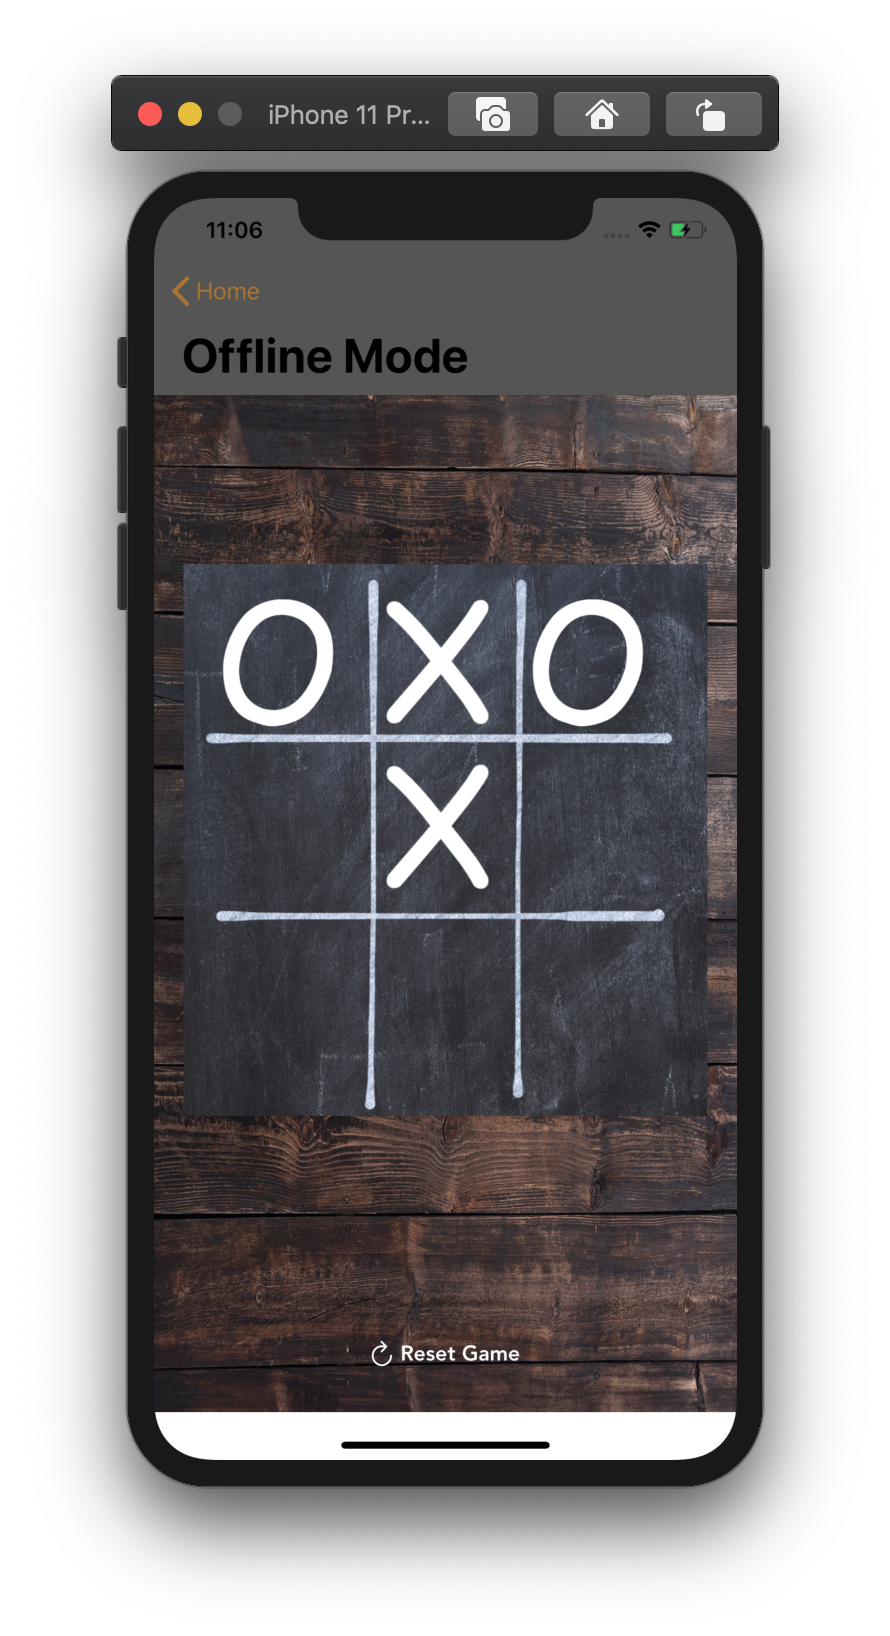
\includegraphics[width=2.5in]{images/board.png}
        \caption{Game Page in Iphone}
        \end{figure}
        ~\newline
        ~\newpage
        
    \subsection{UI Prototype}
        With the given layout, the pages will be designed as shown in below figure
        \begin{figure}[h]
        \centering
        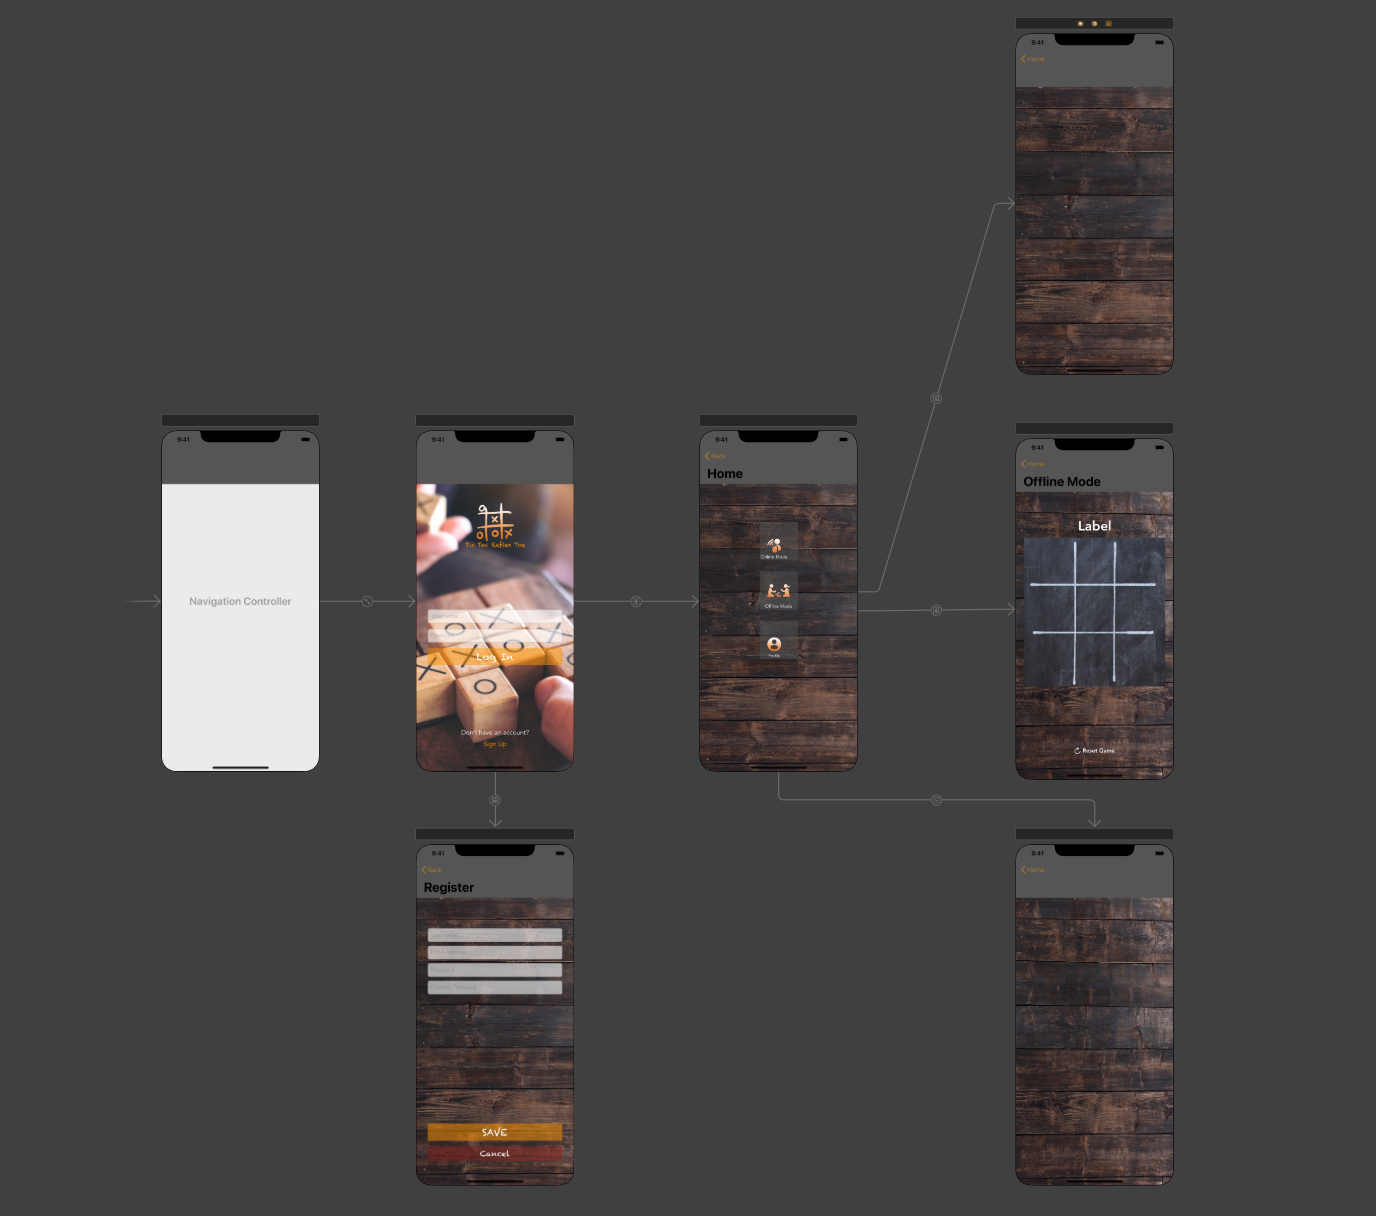
\includegraphics[width=5.5in]{images/Prototype.png}
        \caption{UI Prototype}
        \end{figure}
        ~\newline
        ~\newpage
\newpage

% ****** Project Plan ****** 
\section{Project Plan}
    \subsection{Work Breakdown Structure}
    Below figure shows Work Breakdown Structure for the development of \textbf{\emph{Tic Tac Reflex Toe}}
            \begin{figure}[h]
            \centering
            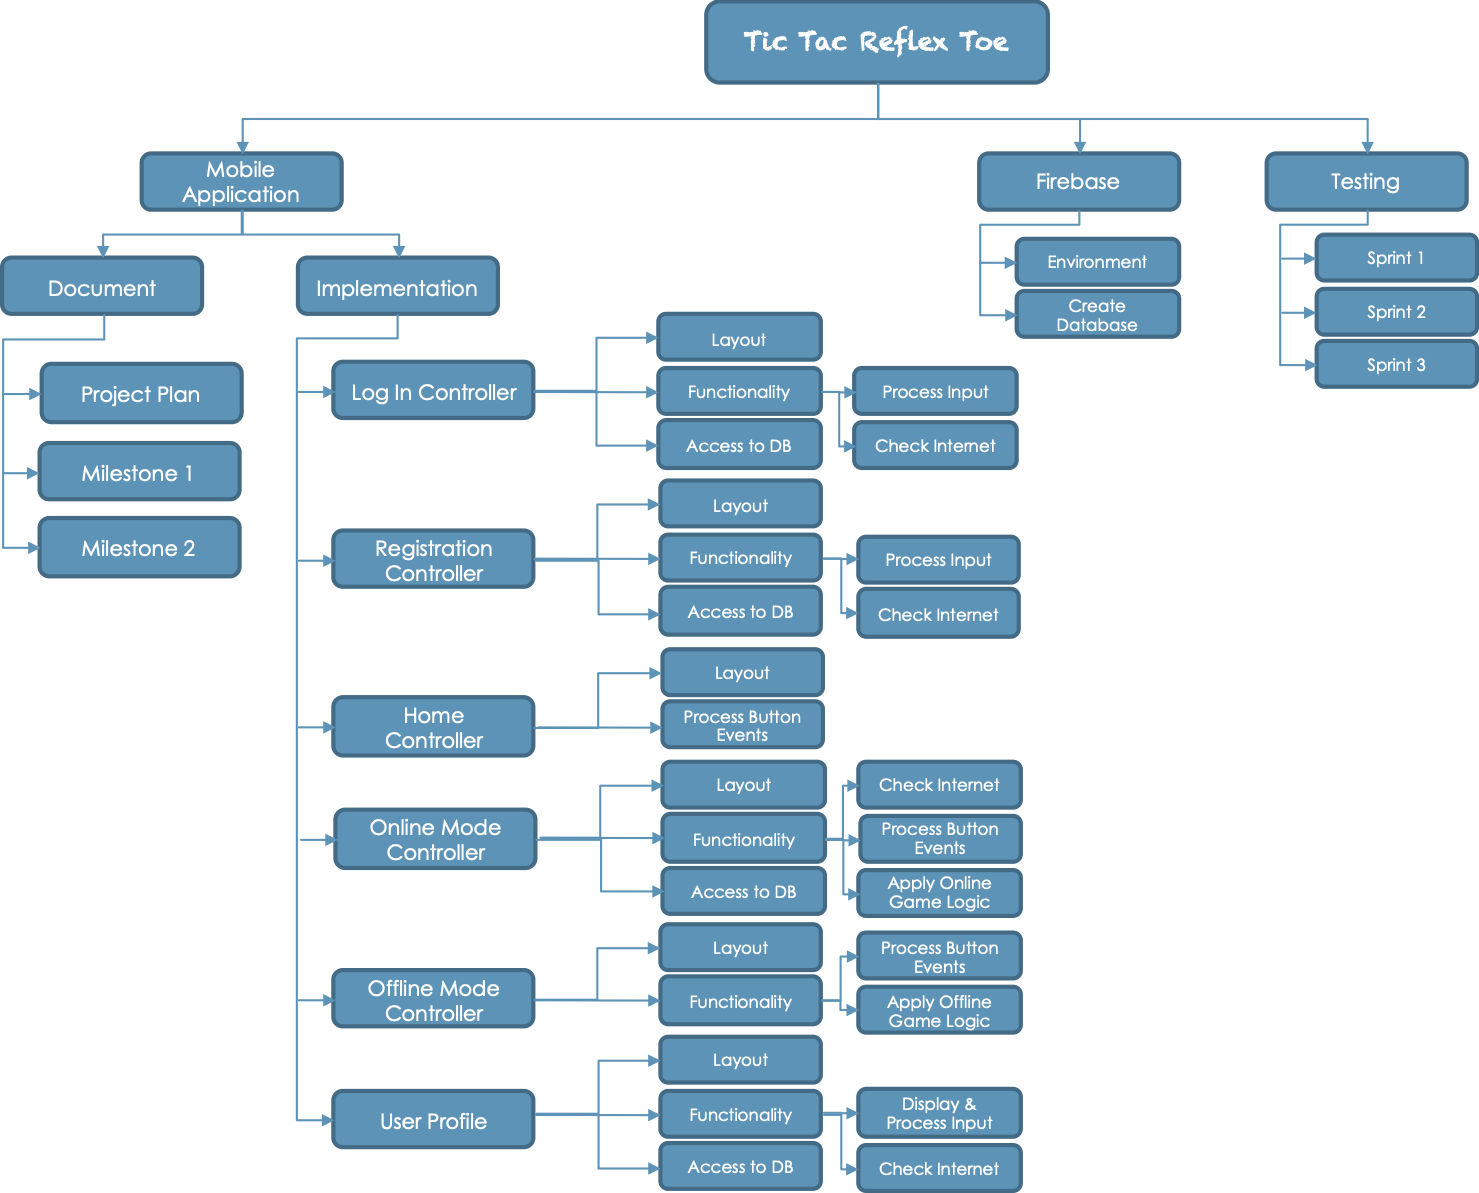
\includegraphics[width=5.5in]{images/Work Breakdown Structure.png}
            \caption{Work Breakdown Structure}
        \end{figure}
        \\
        ~\\
    \subsection{Timeline}
        This project is aimed to finish in time for project scheduled presentation, 24th of August 2020.\\\\
        \subsubsection{Sprint Timeline}
        This will be a Three-Sprint project, each sprint has 3 days and estimated 15 hours per developer on each sprint.\\
        \begin{figure}[h]
        \centering
        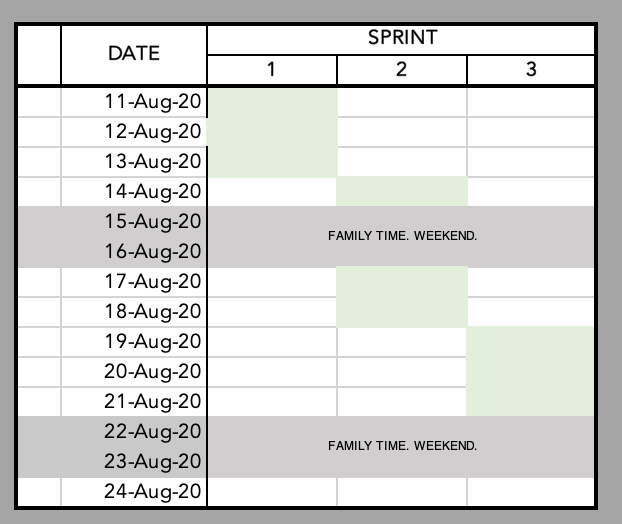
\includegraphics[width=4in]{images/Sprint Timeline.png}
        \caption{Sprint Timeline}
        \end{figure} 
        ~\\
        \newpage
        \subsubsection{Sprint Delivery}
        Each Sprint has specific deliveries in order for the project to be successful.\\
        \begin{figure}[h]
            \centering
            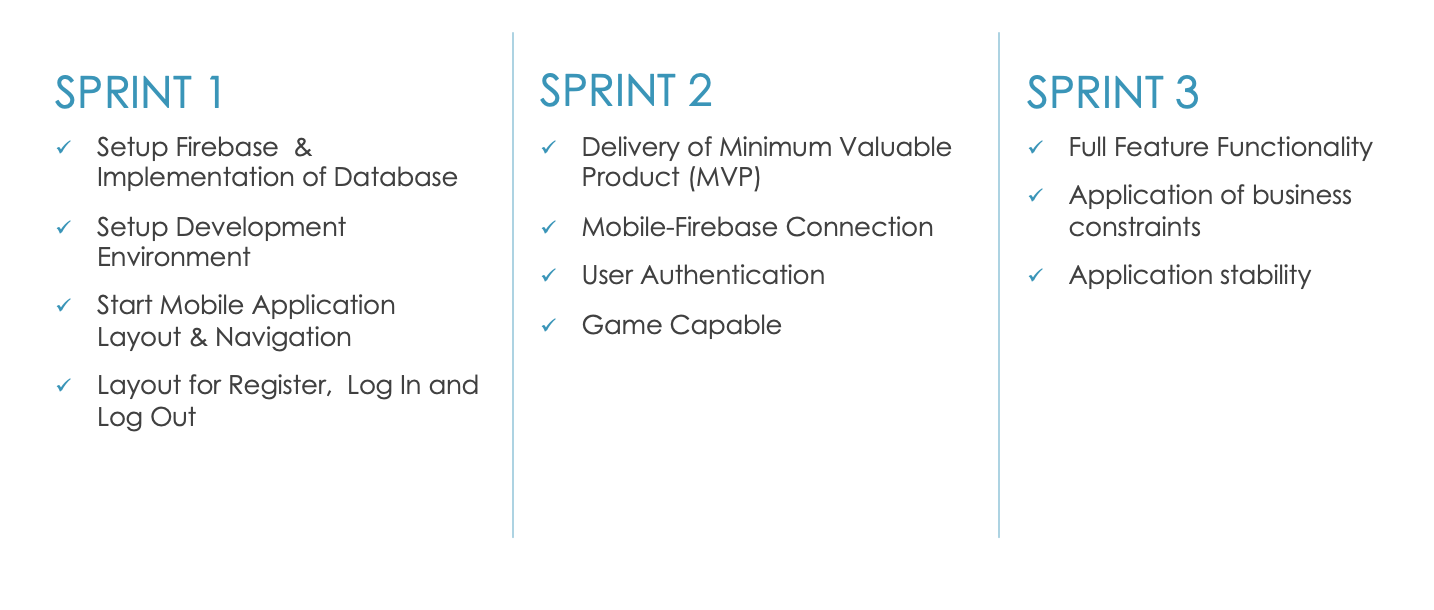
\includegraphics[width=5.5in]{images/Sprint Deliveries.png}
            \caption{Sprint Deliveries}
        \end{figure}
        \\
        ~\\
    \newpage
    \subsection{Tasks Breakdown}
    In order to monitor the project deliveries, the project tasks are broken down to small chunks and are given projected delivery estimation.
        \subsubsection{Gantt Chart}
        Listed below are the tasks broken down to small items and are plotted to sprint dates.  Along with these list are estimated number of hours each task to complete.
        \begin{figure}[h]
            \centering
            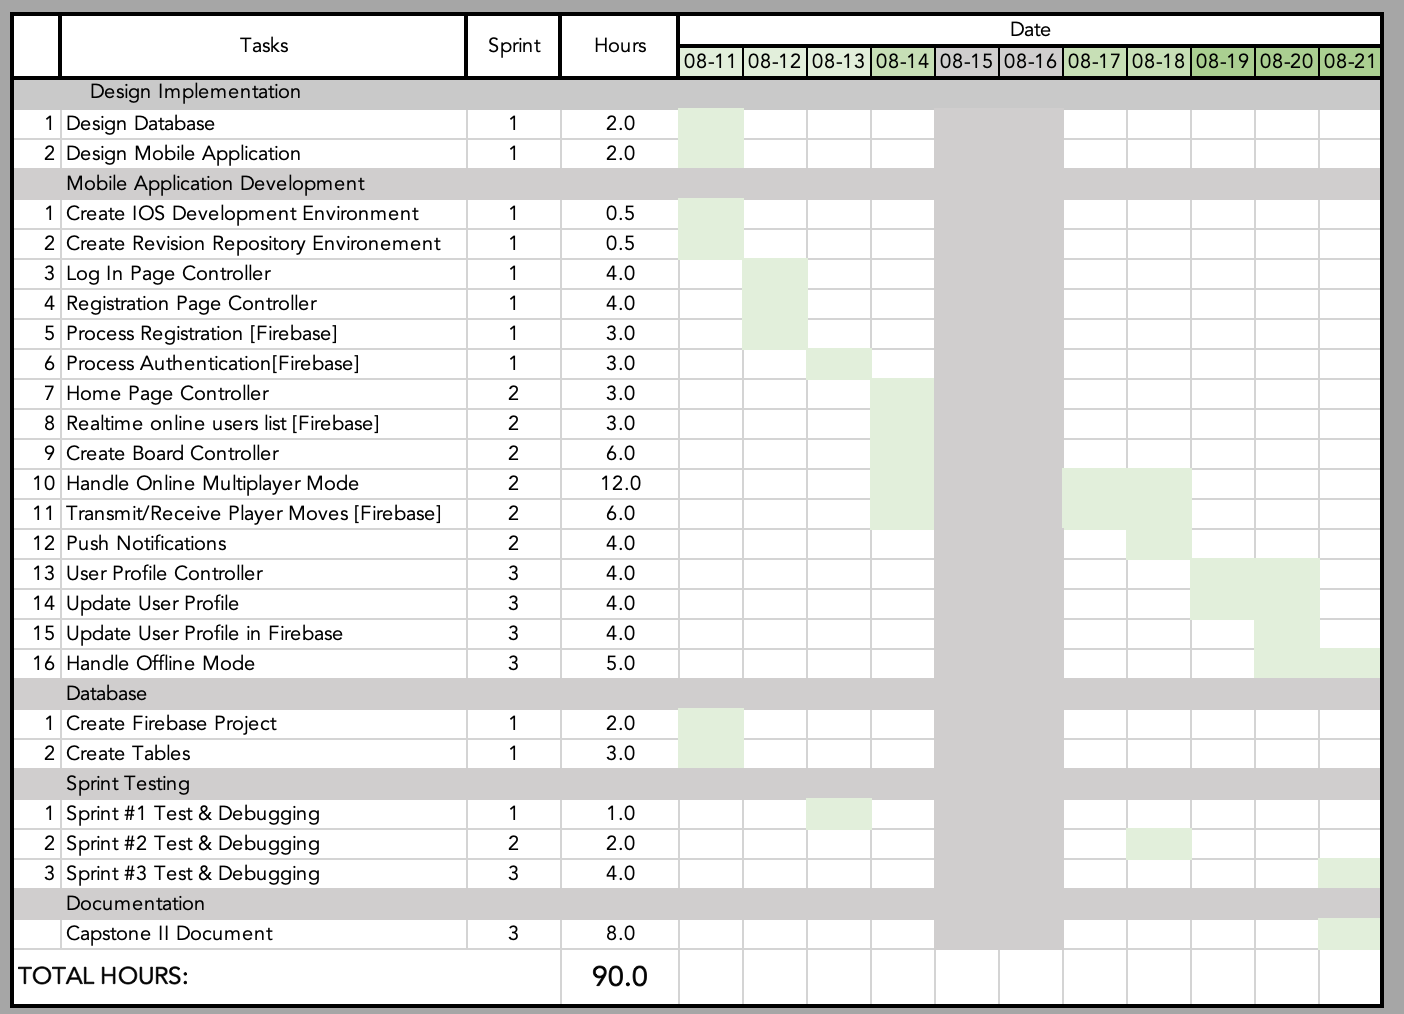
\includegraphics[width=5.5in]{images/Gantt Chart.png}
            \caption{Gantt Chart}
        \end{figure}
        \newpage
        \subsubsection{Critical Path}
        The project is prepared for development worst case schedule to make sure that the project will still be delivered on time.  The best development time projected is only 90.0 hours but with worst case, total development hours would reach to 138.0. To make it possible, weekend work is required.
        \begin{figure}[h]
            \centering
            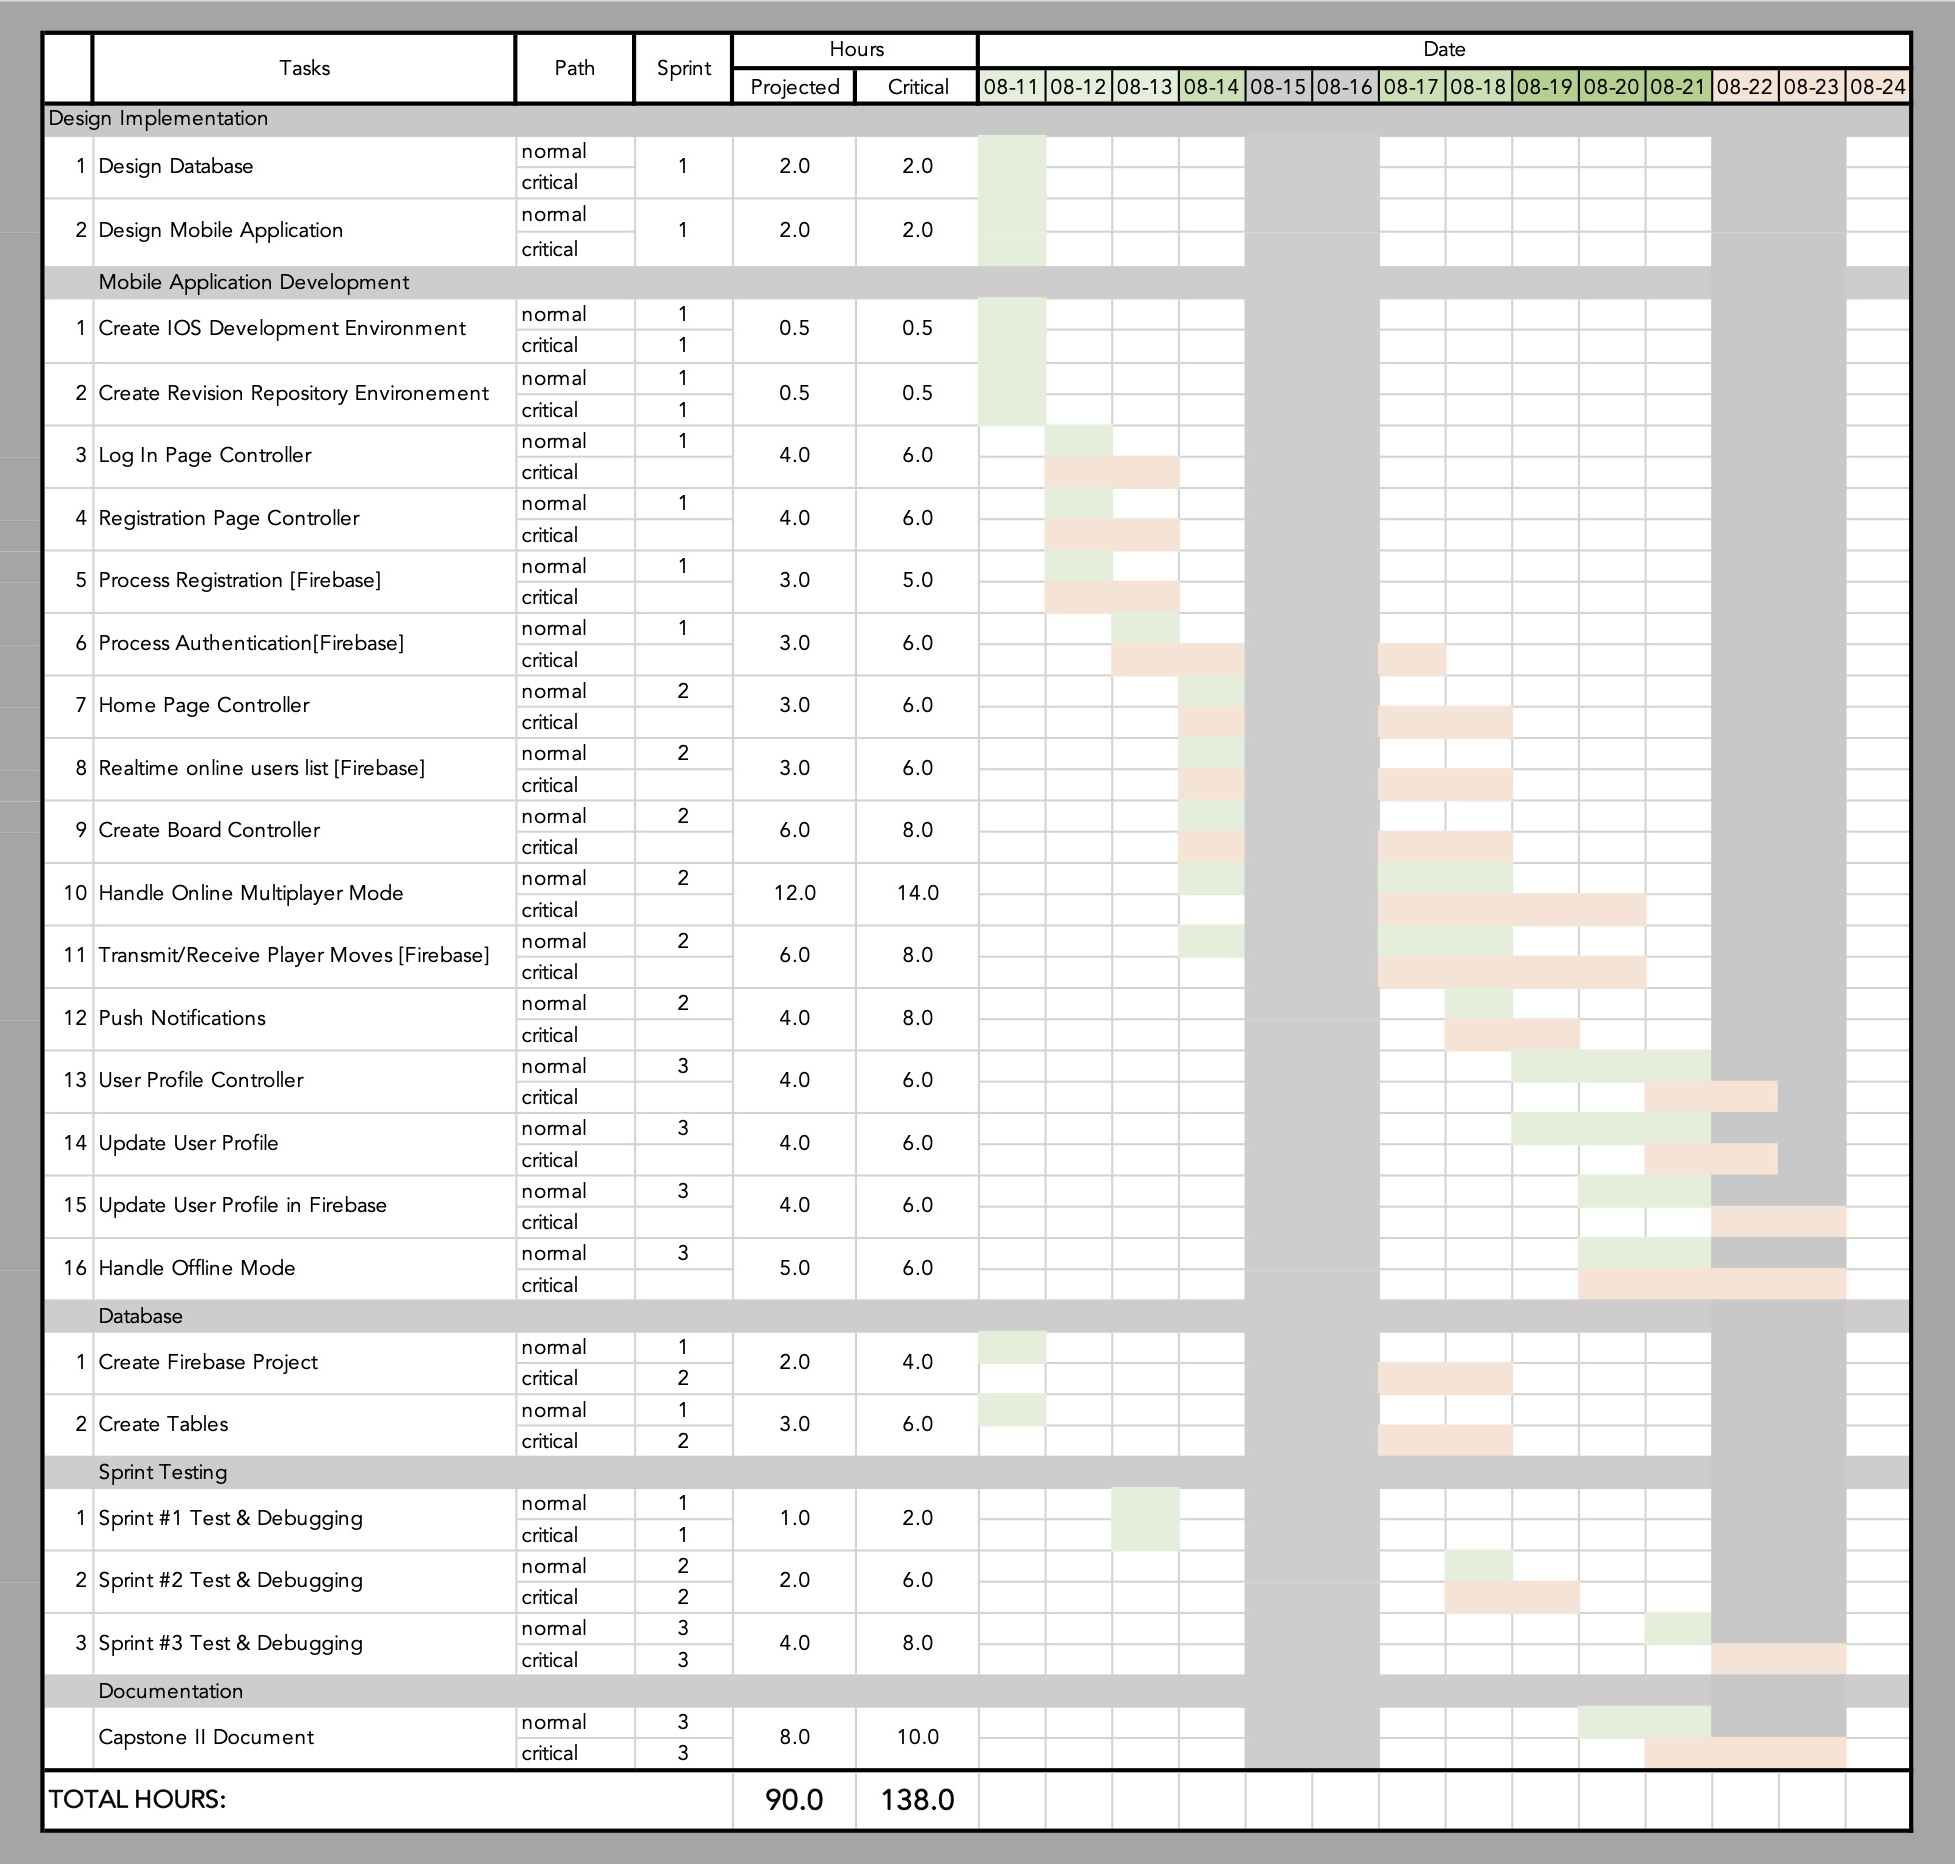
\includegraphics[width=5.5in]{images/Gantt Critical.png}
        \caption{Critical Path}
        \end{figure}
        \newpage
        
        
% ****** ACCEPTANCE PROCEDURE ****** 
\section{Acceptance Procedure}
The following is a checklist that will conclude if the project is complete.  These items listed are functionalities that answers to this projects Users Stories.
    \begin{itemize}
        \item Successful user registration
        \item Successful user log in
        \item Successful user log out
        \item Successful interaction of game play
    \end{itemize}
    ~\\
    
% ****** TOOLS & TECHNOLOGIES ****** 
\section{Tools and Technologies}
    \begin{itemize}
        \item \textbf{XCode 11.4}\\Integrated Development Environment that will be used
        \item \textbf{Swift 5.0}\\Programming language
        \item \textbf{Firebase Realtime Database}\\Stores user data and player actions
        \item \textbf{Photoshop}\\Visuals Editing
        
        \item \textbf{Testing Devices}
            \begin{itemize}
            \item XCode Simulator
            \item IPhone XS Max
            \item IPhone X
            \end{itemize}
    \end{itemize}
\newpage
\section{Implementation}
\subsection{Sprint Retrospectives}
    \subsubsection{Sprint 1}
        \textbf{\emph{What Went Well.}}
        \begin{itemize}
            \item Design and environment setup finished ahead of time
            \item Offline mode was done even it is scheduled for Sprint 3
        \end{itemize}
        \textbf{\emph{What Did Not Go Well.}}
        \begin{itemize}
            \item Some tasks are not finished but worked on the weekend instead
        \end{itemize}
        \textbf{\emph{What Needs Improvement.}}
            \begin{itemize}
                \item Task scheduling
            \end{itemize}~\\
    \subsubsection{Sprint 2}
        \textbf{\emph{What Went Well.}}
        \begin{itemize}
            \item Some tasks are completed as scheduled
        \end{itemize}
        \textbf{\emph{What Did Not Go Well.}}
        \begin{itemize}
            \item Schedules are tight and documentation is not taken to consideration in Sprint planning
            \item MVP is not delivered
        \end{itemize}
        \textbf{\emph{What Needs Improvement.}}
            \begin{itemize}
                \item Task scheduling
            \end{itemize}~\\
    \subsubsection{Sprint 3}
        \textbf{\emph{What Went Well.}}
            \begin{itemize}
                \item Tasks are completed.  Project functional.
            \end{itemize}
        \textbf{\emph{What Did Not Go Well.}}
            \begin{itemize}
                \item Although the features are functional it is not Regression tested.
            \end{itemize}
        \textbf{\emph{What Needs Improvement.}}
            \begin{itemize}
                \item Stability and more visuals to make the app interesting
            \end{itemize}

\newpage
\subsection{Tasks Hours}
The following Gantt Chart shows comparison of projected hours estimated for a task and date it is scheduled to be implemented.  Although Sprint schedule was not religiously followed, the development is still a success since some tasks are developed ahead, and there are buffer days available like weekends.  
        \begin{figure}[h]
            \centering
            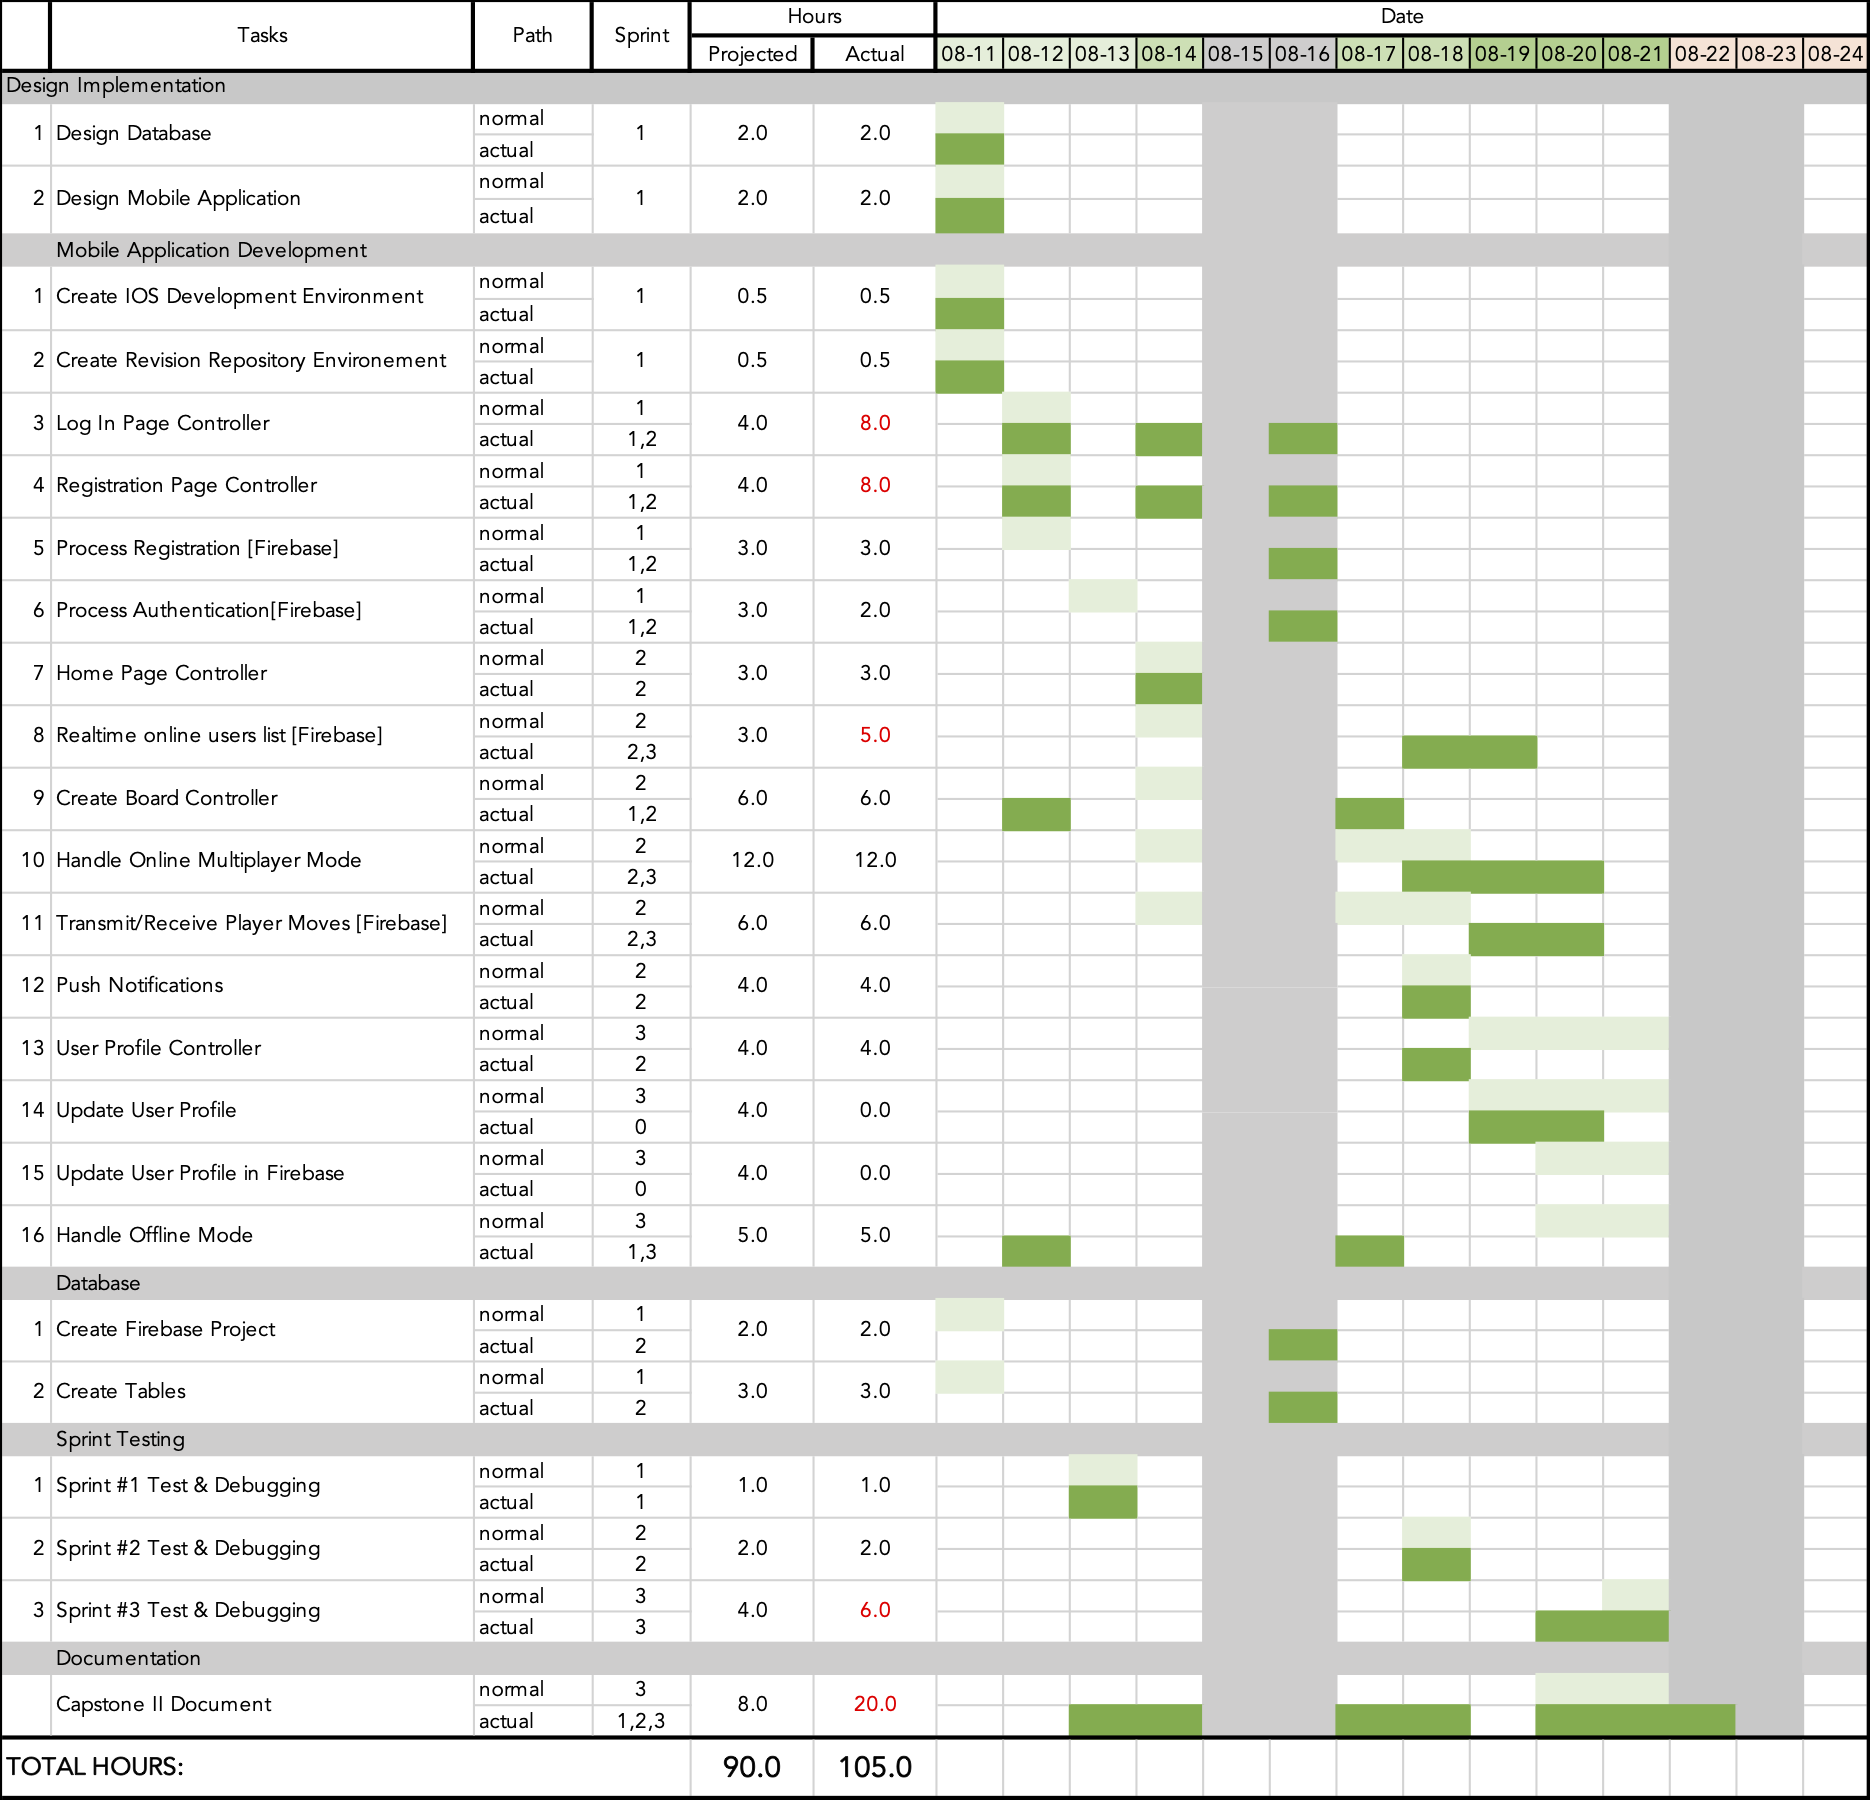
\includegraphics[width=5.5in]{images/Gantt Actual.png}
        \caption{Gantt Chart with Actual Hours}
        \end{figure}
        \newpage  
\newpage
\subsection{Implementation Functions}
    \subsubsection{Database}
    The database contains user class details.  User data is stored in Google Firebase.
        \begin{figure}[h]
            \centering
            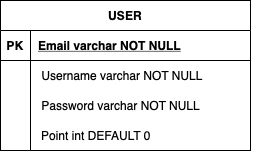
\includegraphics[width=3in]{images/TTRT.png}
        \caption{User Class Diagram}
        \end{figure}
        \newpage   
    \subsubsection{Log In}
    Log In is a separate View Controller Class with the following available user inputs:
        \begin{figure}[h]
            \centering
            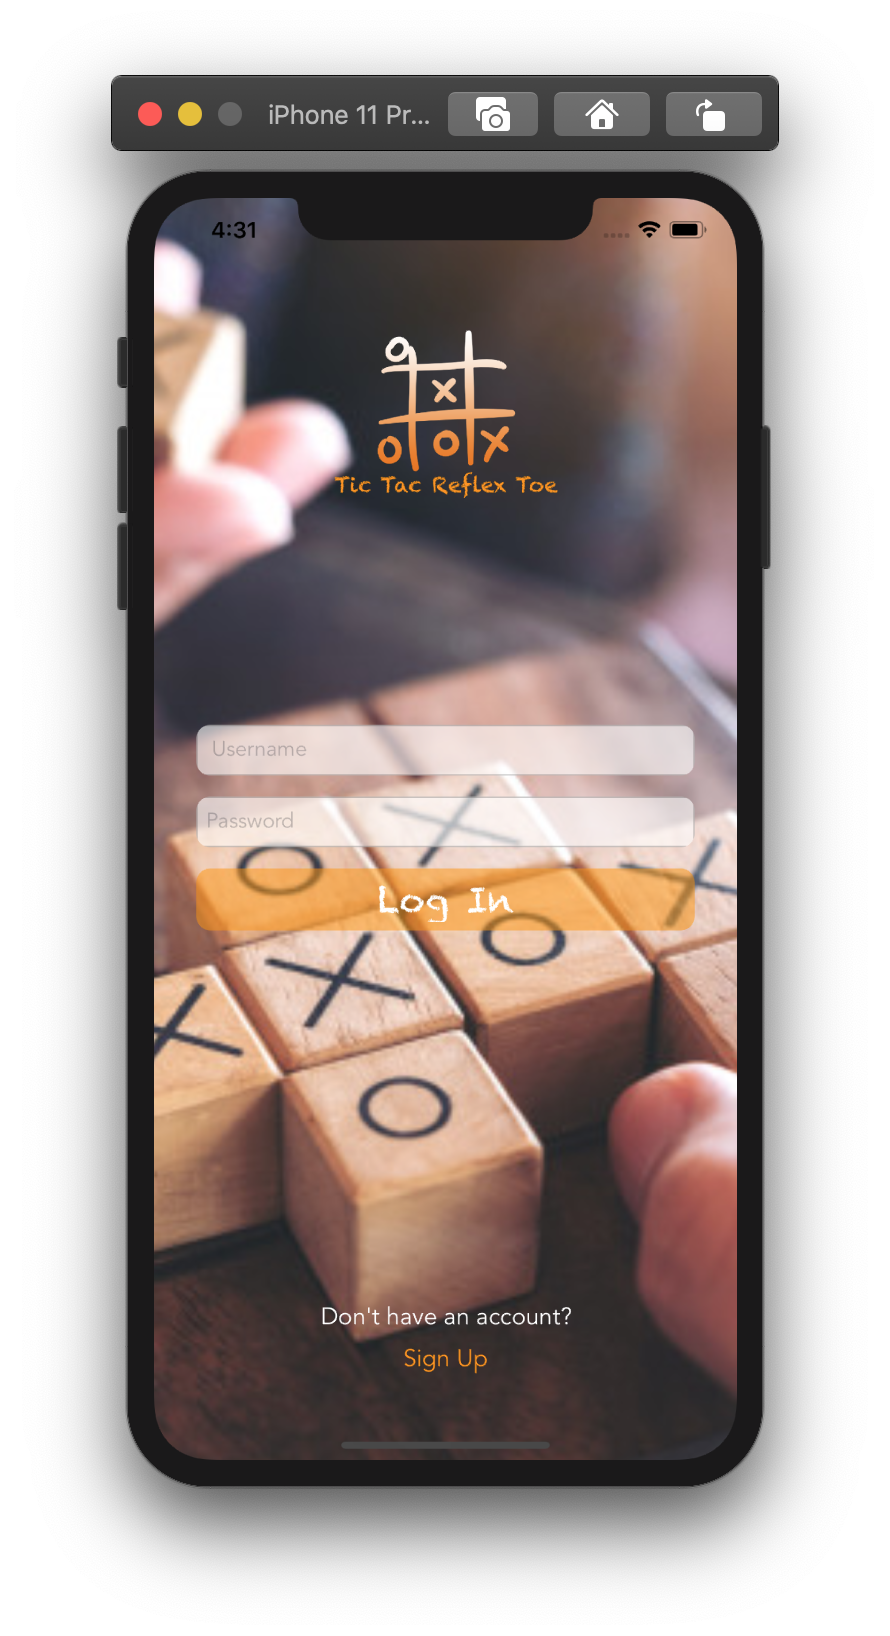
\includegraphics[width=2in]{images/sim_log.png}
        \caption{Actual Log In Page on XCode Simulator}
        \end{figure}
        \newline
        \begin{itemize}
            \item User Text Input - The user email used in the registration of the App
            \item Password Text Input - Must be at least 6 digit.  Entry is secured
            \item Log In Button - To confirm user log in
            \item Sign Up Button - For new users to register a new account.  This will display Register Page Controller
        \end{itemize}
        \newpage
    \subsubsection{Register}
        Register Page is implemented in View Controller Class that handles user sign ups.  Field contents are checked to make sure all are filled and passwords matched to make sure on a successful registration.
        \begin{figure}[h]
            \centering
            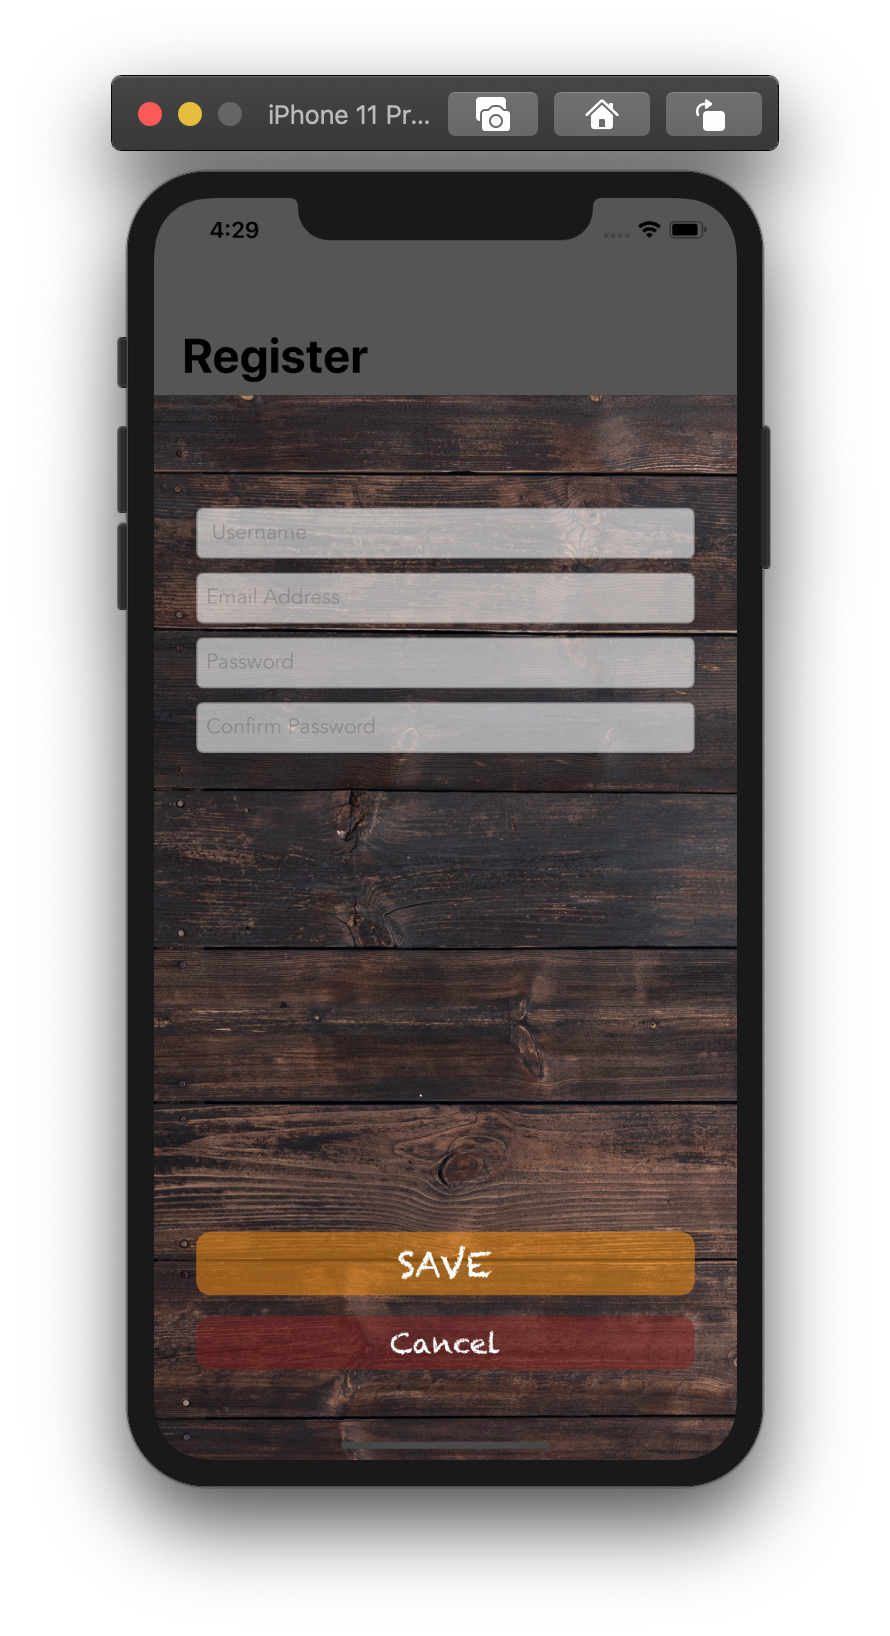
\includegraphics[width=2in]{images/sim_reg.png}
        \caption{Actual Register Page on XCode Simulator}
        \end{figure}
        \newline
        \begin{itemize}
            \item User Name Text Input - User's username
            \item User Email Text Input - The user email and this will be used as a log in credential
            \item Password Text Input - Must be at least 6 digit.  Entry is secured
            \item Confirm Password Text Input - Confirms password entered
            \item Save Button - Confirms registration
            \item Cancel Button - Cancels registration
        \end{itemize}
        \newpage
    \subsubsection{Home Dashboard}
        Home is a implemented using View Controller Class with three main buttons to traverse to different pages
        \begin{figure}[h]
            \centering
            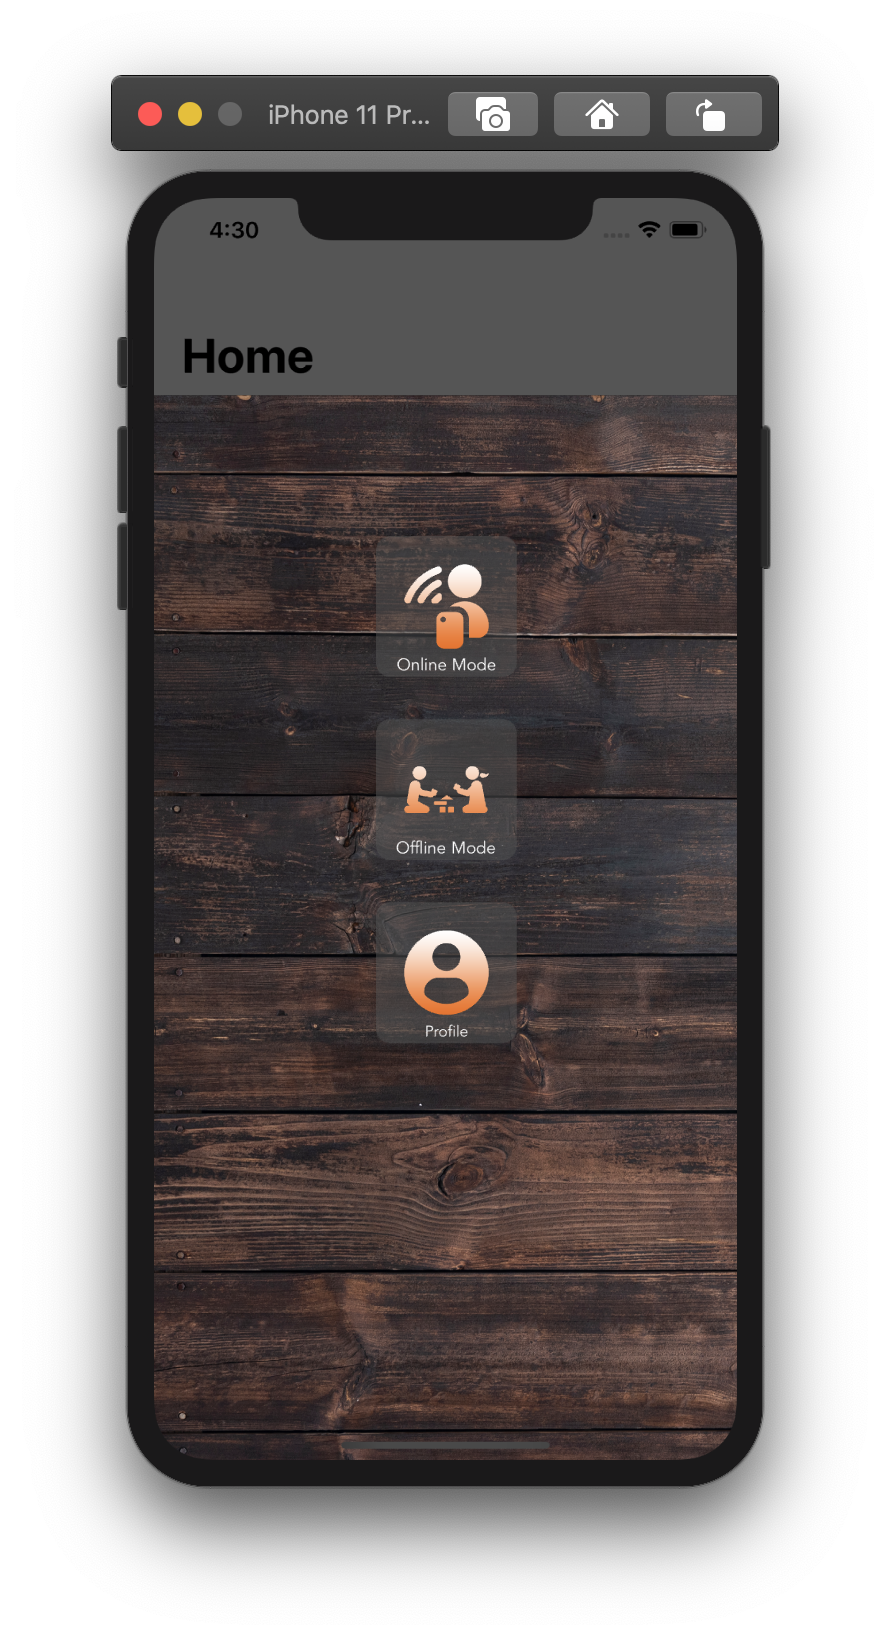
\includegraphics[width=2in]{images/sim_home.png}
        \caption{Actual Home Page on XCode Simulator}
        \end{figure}
        \newline
        \begin{itemize}
            \item Online Mode Button - This option will let the user play in online mode
            \item Offline Mode Button - This option will let the user play in offline mode
            \item User Profile Button - This will display user profile information
        \end{itemize}
        \newpage
    \subsubsection{Offline Game Mode}
    This page is implemented using a View Controller class.  The offline mode gives the user the privilege to enjoy Tic Tac Reflex Toe offline with opponents that are physically present.  The points earned in this mode will not be counted to user over all points.  The bottom button allows the user to Reset the ongoing game or play again if the game finishes.
        \begin{figure}[h]
            \centering
            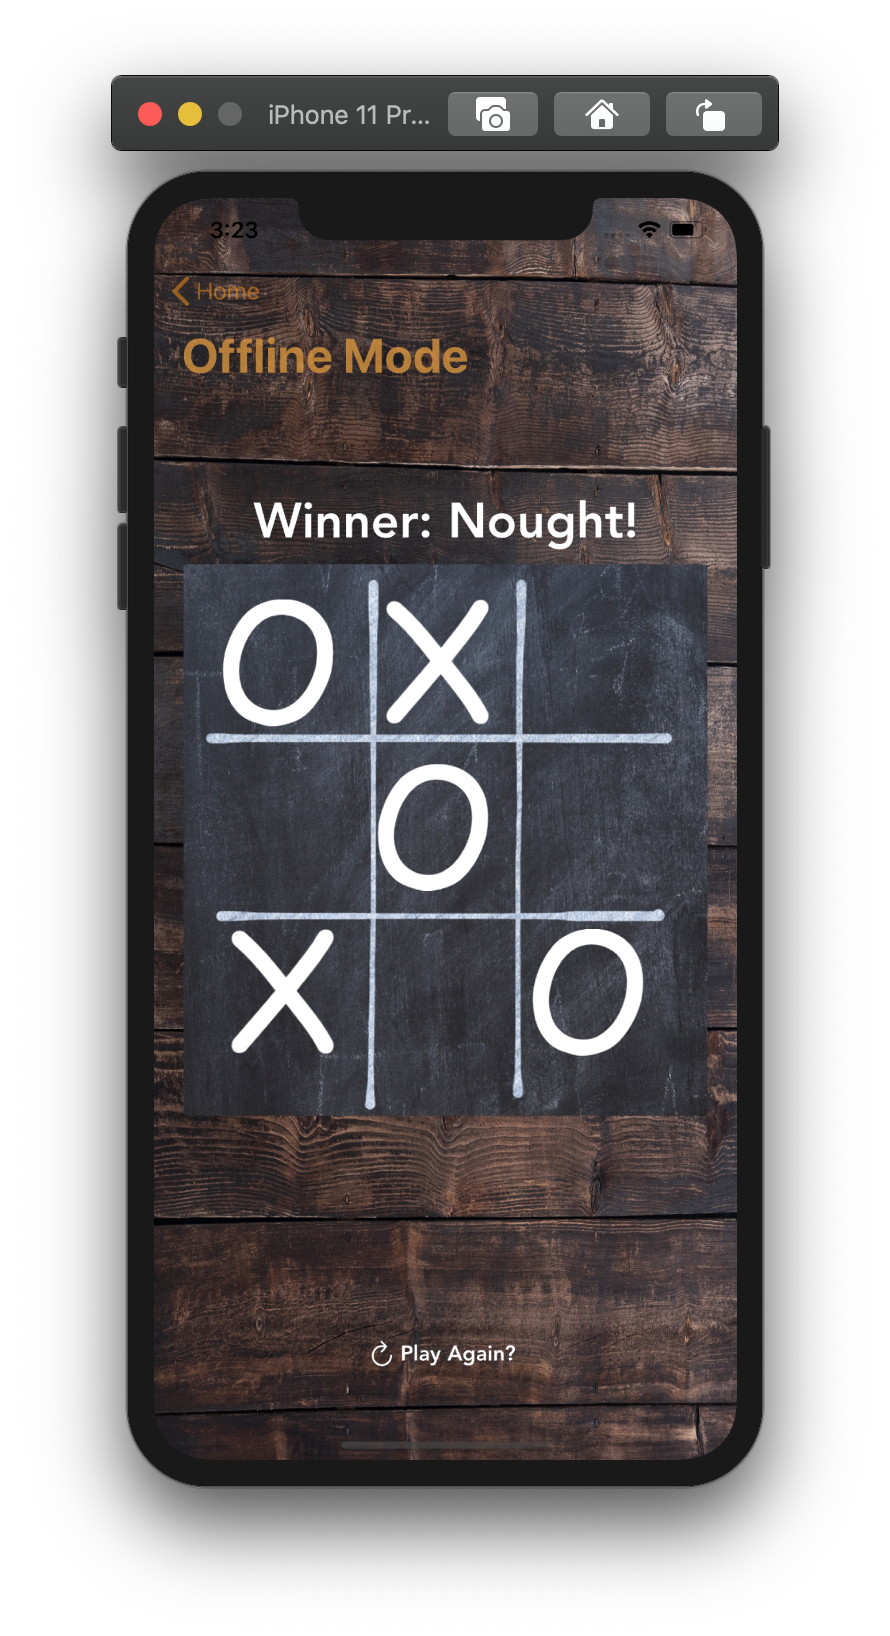
\includegraphics[width=2in]{images/sim_off.png}
        \caption{Actual Offline Game Page on XCode Simulator}
        \end{figure}  
        \newpage
    \subsubsection{Online Game Mode}
    This is the main feature of the App.  This allows user to play Tic Tac Reflex to with  online opponents.  When clicking button online game, the user will see available rooms or create a new room to play the game as seen in the left figure below.  Once in game mode, the game will start as soon as an opponent joins the game.
            \begin{figure}[h]
            \centering
            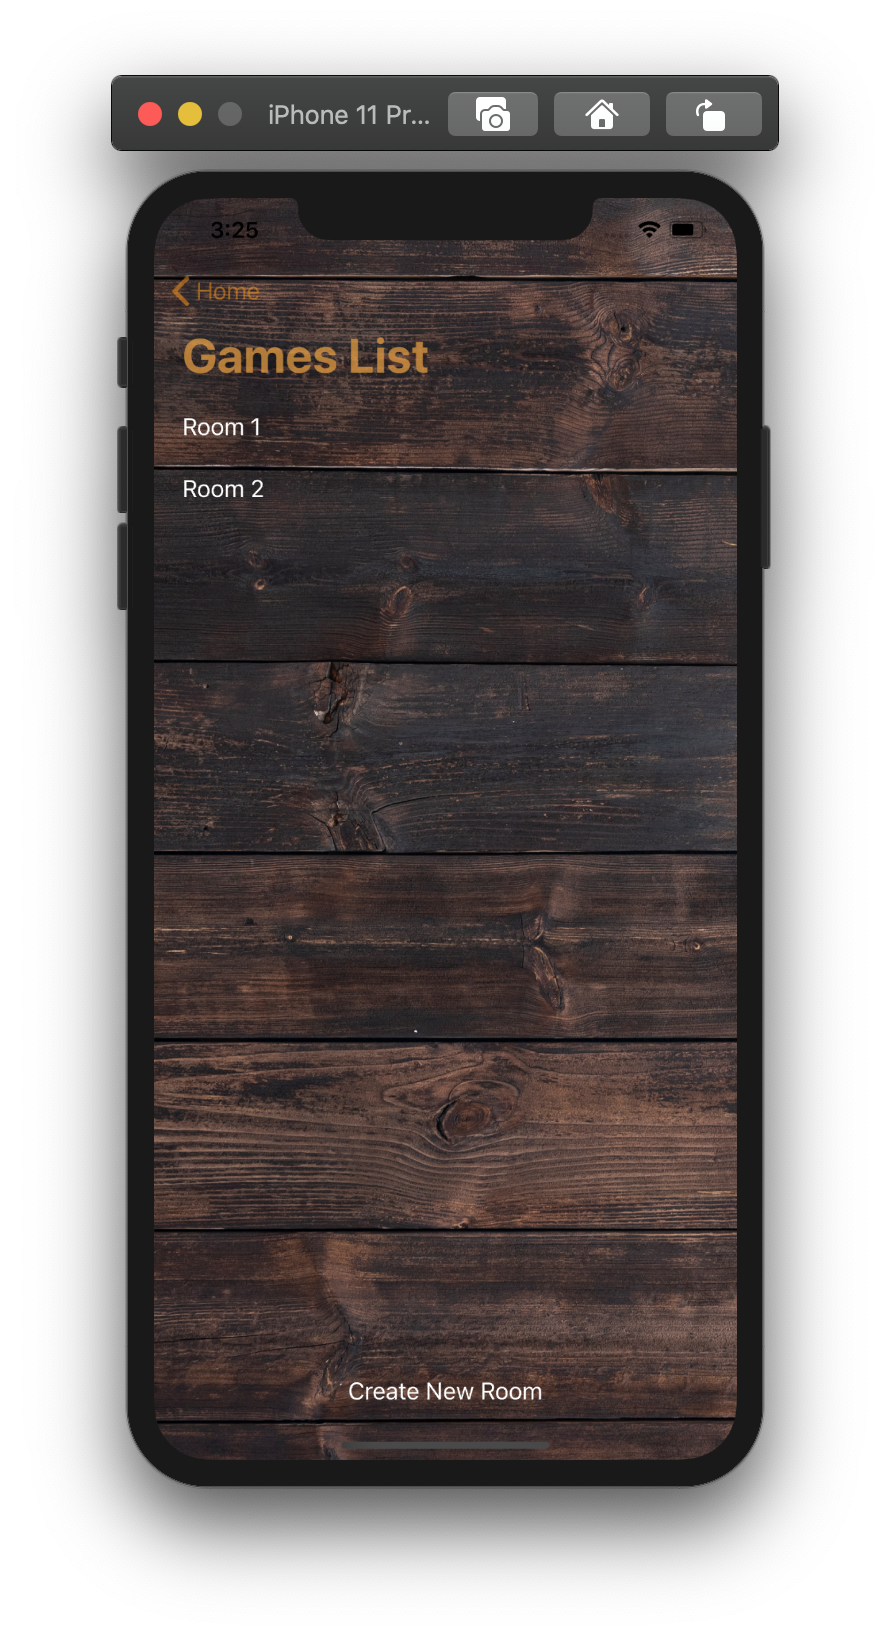
\includegraphics[width=2in]{images/sim_room.png}
            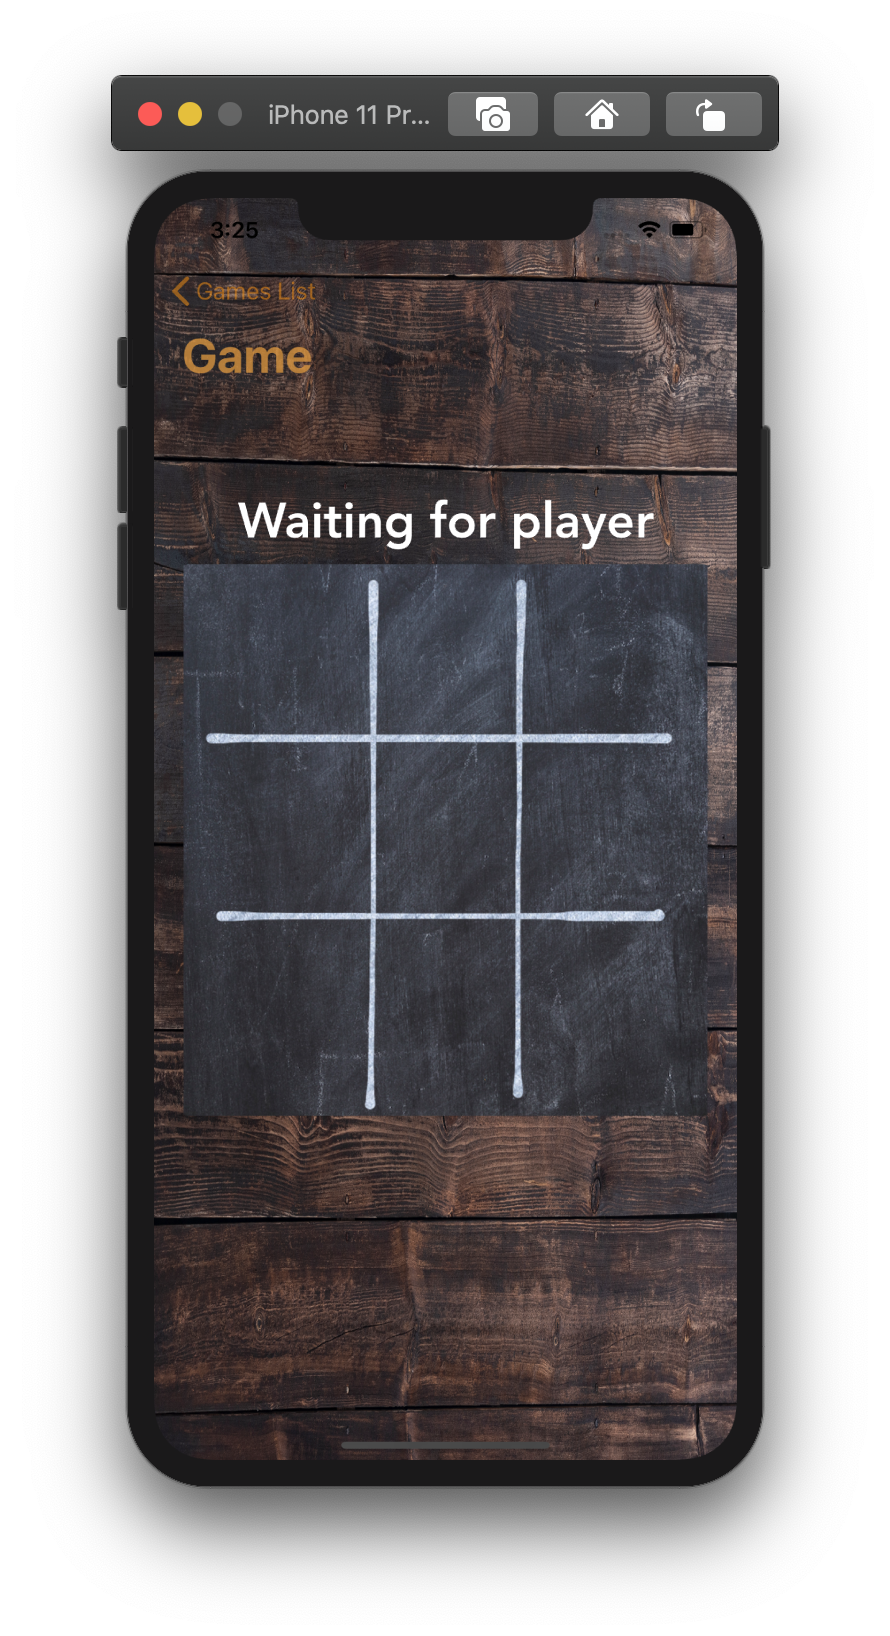
\includegraphics[width=2in]{images/sim_on.png}
        \caption{Actual Online Game Pages on XCode Simulator}
        \end{figure}  
        \newpage
    \subsubsection{User Profile}
    This page is implemented using a View Controller class.  This displays user class information such as name, email, and score in a form of text fields.  A button is available to allow user to sign out.
        \begin{figure}[h]
            \centering
            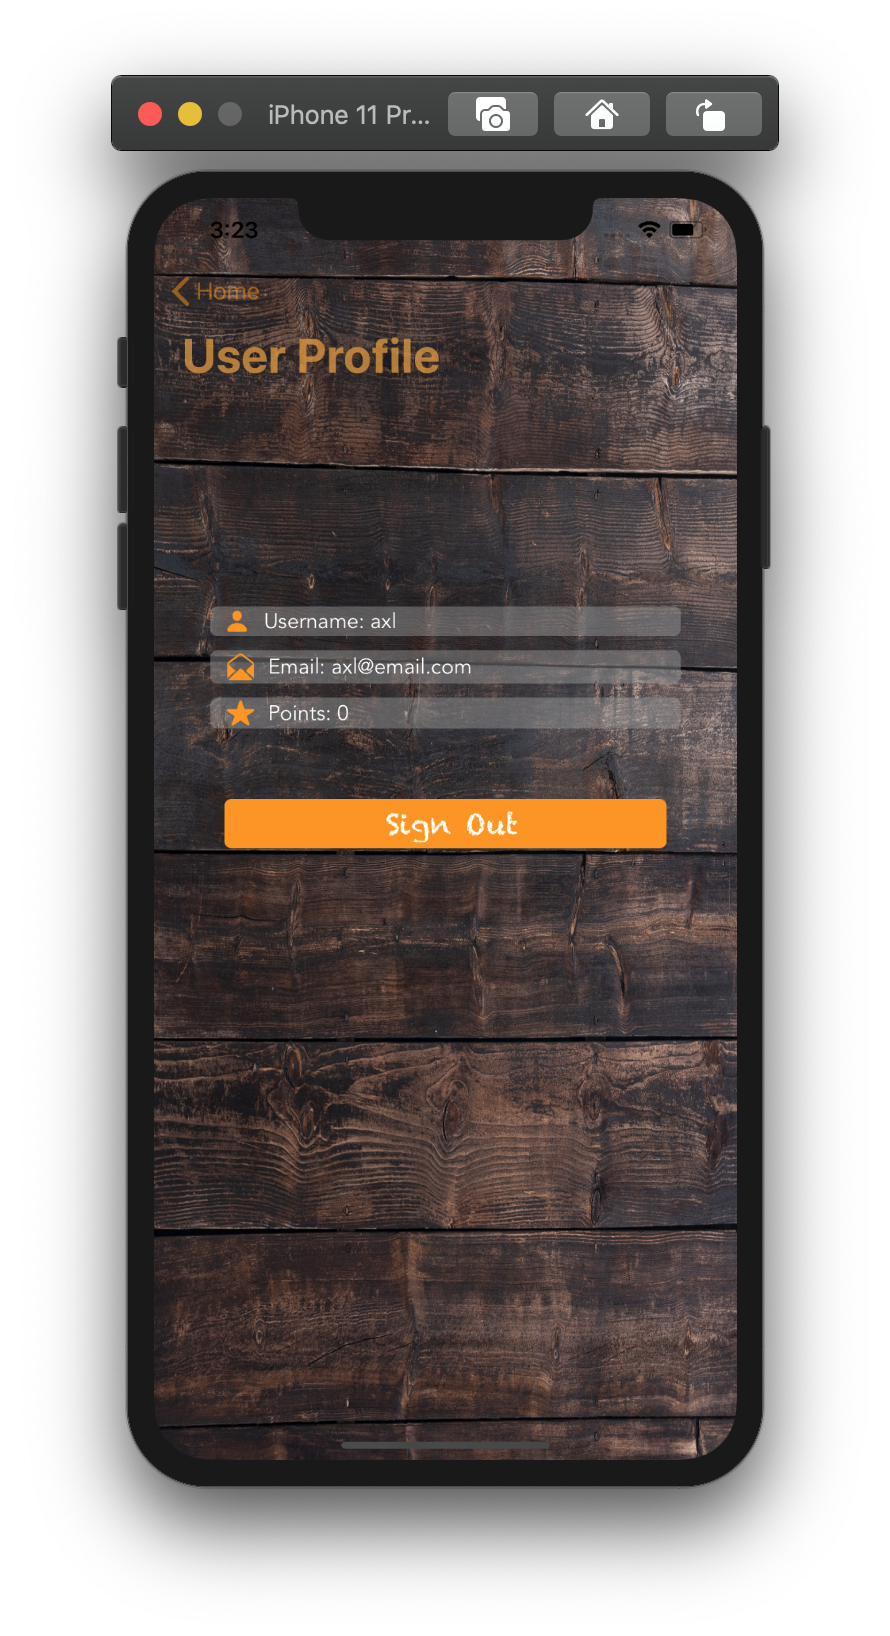
\includegraphics[width=2in]{images/sim_user.png}
        \caption{Actual User Profile Page on XCode Simulator}
        \end{figure}  

\newpage
\subsection{Definition of Done} This section shows the test results of the application functionality which concludes if it has function as planned.
    \subsubsection{Installation}
         \begin{figure}[h]
            \centering
            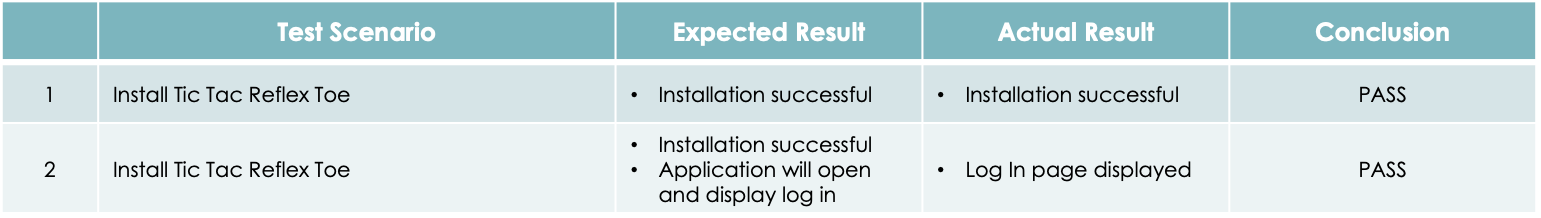
\includegraphics[width=5.5in]{images/test_1_install.png}
        \caption{Installation Test Cases}
        \end{figure}   
    \subsubsection{Log In}
        \begin{figure}[h]
            \centering
            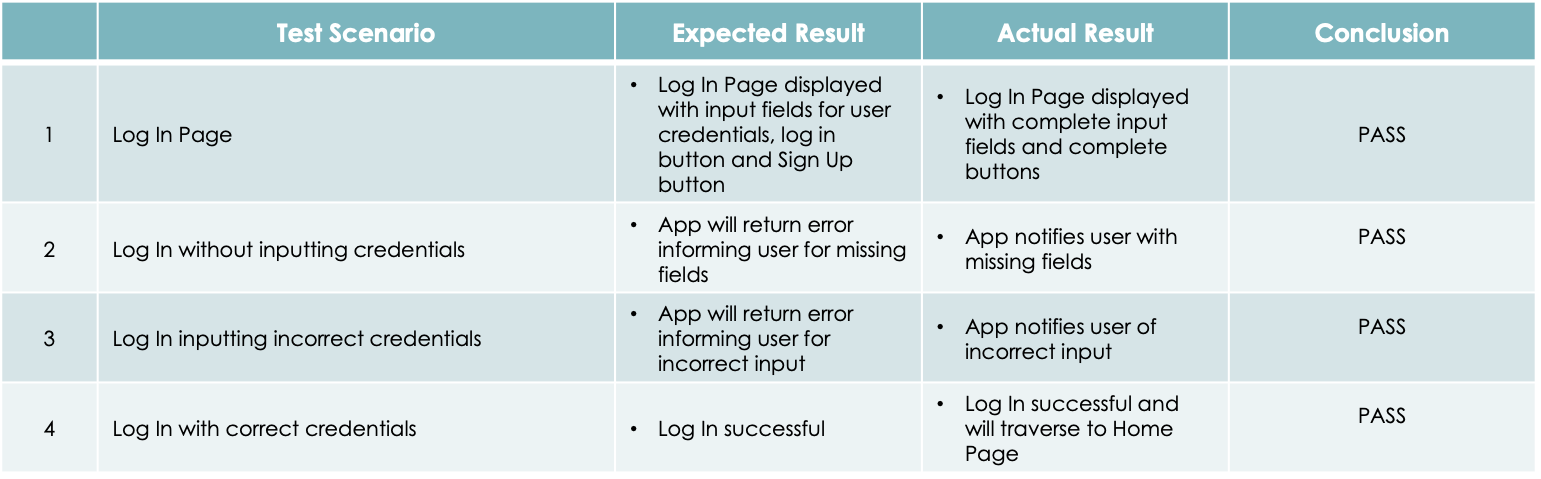
\includegraphics[width=5.5in]{images/test_2_log.png}
        \caption{Log In Test Cases}
        \end{figure}
        \newpage
    \subsubsection{Register}
        \begin{figure}[h]
            \centering
            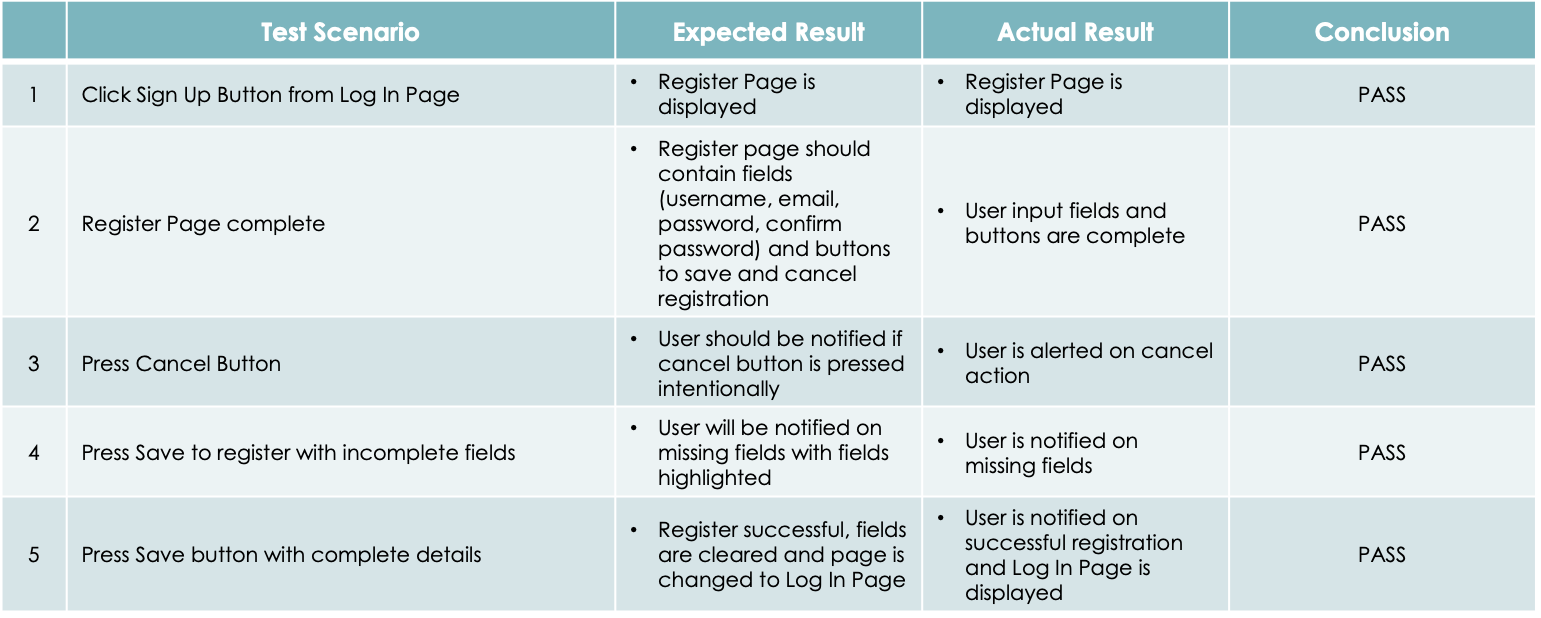
\includegraphics[width=5.5in]{images/test_3_register.png}
        \caption{Register Test Cases}
        \end{figure}
    \subsubsection{Home Dashboard}
        \begin{figure}[h]
            \centering
            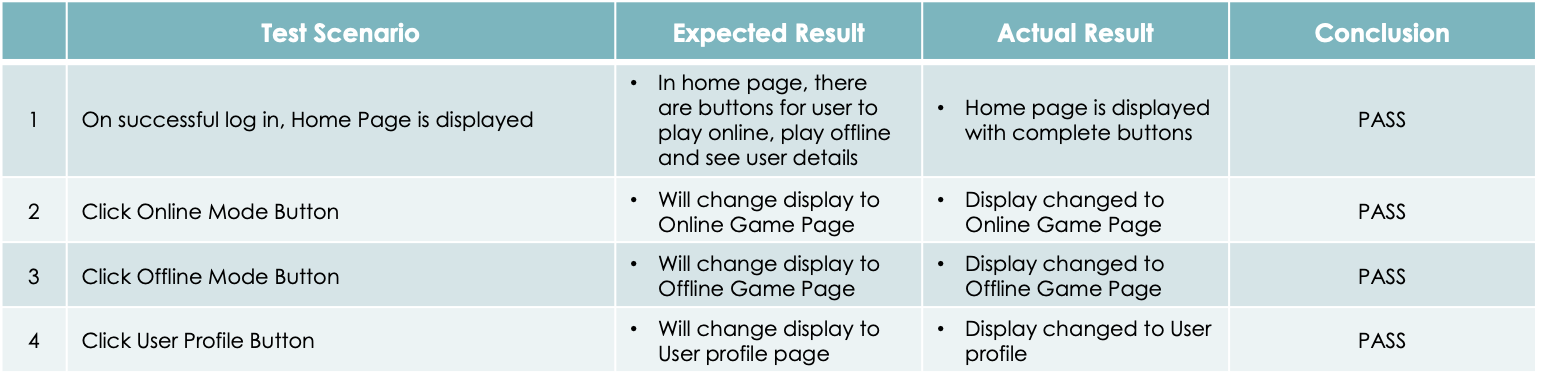
\includegraphics[width=5.5in]{images/test_4_home.png}
        \caption{Home Page Test Cases}
        \end{figure}
        \newpage
    \subsubsection{Online Game Mode}
        \begin{figure}[h]
            \centering
            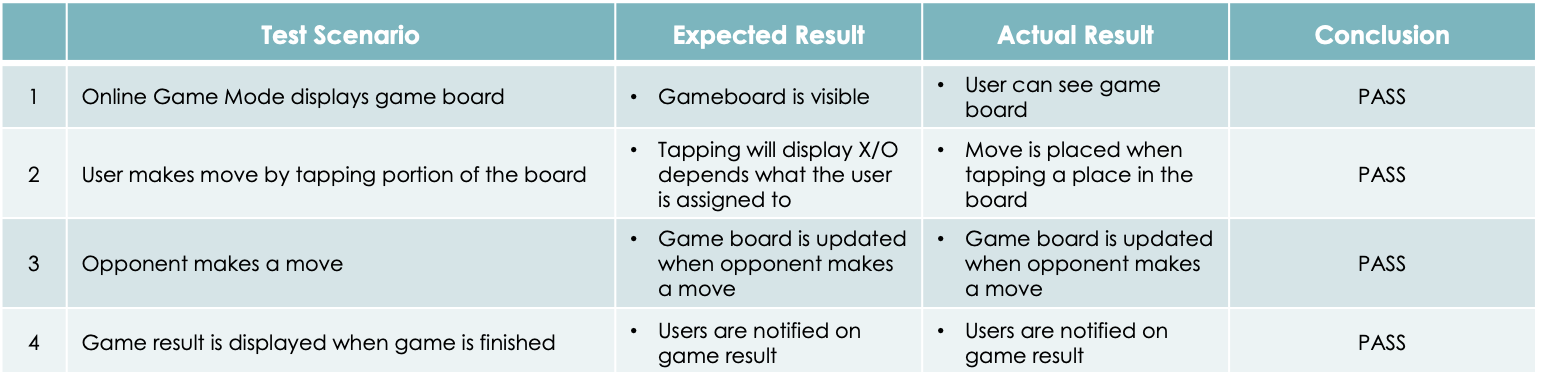
\includegraphics[width=5.5in]{images/test_5_online.png}
        \caption{Online Game Mode Page Test Cases}
        \end{figure}
    \subsubsection{Offline Game Mode}
        \begin{figure}[h]
            \centering
            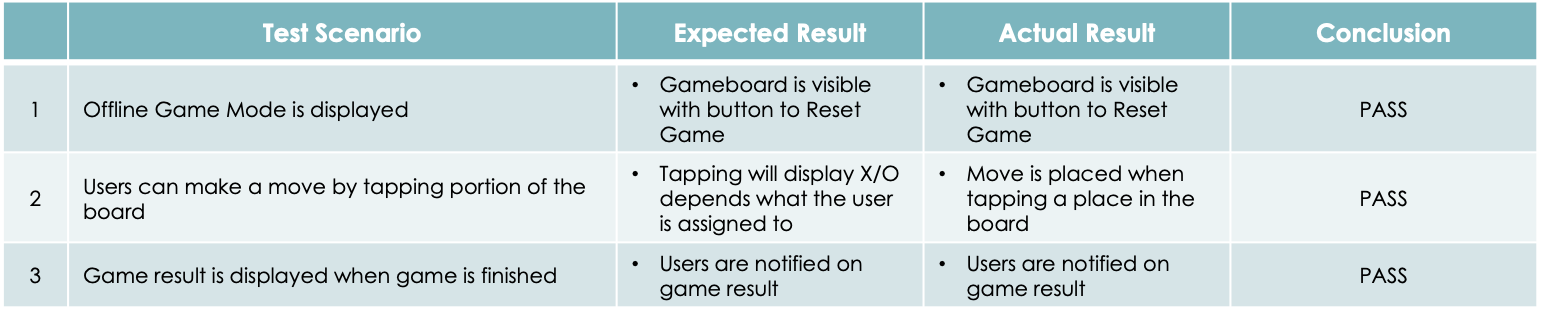
\includegraphics[width=5.5in]{images/test_6_offline.png}
        \caption{Offline Game Mode Page Test Cases}
        \end{figure}
    \subsubsection{User Profile}
        \begin{figure}[h]
            \centering
            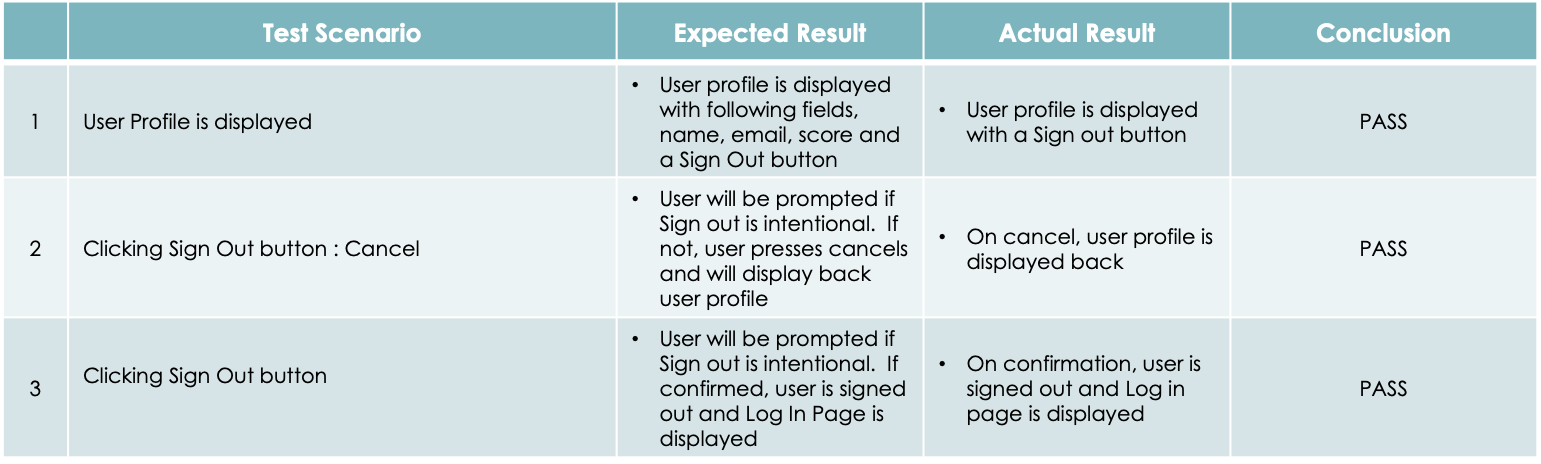
\includegraphics[width=5.5in]{images/test_7_profile.png}
        \caption{User Profile Page Test Cases}
        \end{figure}
    \newpage
\section{Improvements}
There are many ways to improve \textbf{\emph{Tic Tac Reflex Toe}} and listed are the few things current development can think of
\begin{itemize}
    \item Profile Picture\\
    It is nice having to have a profile picture assigned to user
    \item Log In Using Social Media\\
    Like most applications, you can register using Facebook and Google accounts
    \item Friend List\\
    Adding your favorite opponent to friend list
    \item Online Notifications\\
    Be notified for news, updates, tournaments and even when your favorite opponent is online
    \item Chat\\
    Be able to chat your friends
    \item Share in social media
    Be able to post game victories in Social Media like Facebook or Instagram.  This feature would be a help for marketing
    \item Cross Platform Support
    Be able to support \textbf{\emph{Tic Tac Reflex Toe}} for Android
\end{itemize}
\section{Links}
\begin{itemize}
    \item Github Link:\\ \url{https://github.com/otetLopez/TicTacReflexToe/}
    \item Video Demo:\\
    \url{https://github.com/otetLopez/TicTacReflexToe/Video}
    \item Google Site:\\
    \url{https://sites.google.com/view/tic-tac-reflex-toe/home}
    \item Latex Overleaf Link:\\
    \url{https://www.overleaf.com/read/jvysgmwscznm}
\end{itemize}
\newpage

\section{Bibliography}
\end{document}


